\documentclass{brownthesis}
\usepackage{amsmath}
\usepackage{amssymb}
\usepackage{graphicx}
\usepackage{tikz}
\usepackage{bbm}
\usepackage{verbatim}
\usepackage[percent]{overpic}

\DeclareMathOperator{\Tr}{tr}
\DeclareMathOperator{\tr}{tr}
\DeclareMathOperator*{\diag}{diag}
\DeclareMathOperator{\arctanh}{arctanh}
\DeclareMathOperator{\arcsinh}{arcsinh}
\DeclareMathOperator{\sech}{sech}
\DeclareMathOperator{\var}{var}

\def\dd{{\rm d}}
\def\LL{{\rm L}}
\def\RR{{\rm R}}

\begin{document}

\title{\say{A Tale of 2-Spheres}: How Conformal Symmetry, Chaos, and\\
  Some Elementary Algebra Led to Insights in\\
  Black Holes and Quantum Cosmology}
\author{Chang Liu}
\degrees{B.~Sc., University of Science and Technology of China, 2013\\
  M.~Eng., University of Auckland, 2015\\
  M.~Sc., University of Auckland, 2017\\
  M.~Sc, Brown University, 2019}
\principaladvisor{David Anthony Lowe}
\reader{David Anthony Lowe}
\reader{Antal Jevicki}
\reader{Stephon Haigh-Solomon Alexander}
\dean{Andrew G.~Campbell}
\abstract{The unification of quantum mechanics and general relativity is the holy grail of fundamental theoretical physics. This thesis represents a small part of that effort, where we consider a number of problems that might be of interest to the theoretical studies of black holes and quantum cosmology. Why study black holes and quantum cosmology, one might ask? The answer lies in the fact that they are the only two systems where it is necessary to apply quantum mechanics and general relativity simultaneously. In particular, they both have event horizons, which are global structures of the spacetime that prevent events from making causal contact. They therefore have become the primary arenas where logical incompatibilities of quantum mechanics and general relativity can be made most transparent. One of the most dramatic incompatibilities is the black hole information paradox, which concerns the unitarity of processes that involve the formation and the evaporation of black holes. This thesis will first discuss a proposed resolution to the information paradox called black hole complementarity, and a closely linked issue known as quantum scrambling, in particular in the context of a 2D conformal field theory. We will then present a microscopic quantum model of the de-Sitter universe that incorporates the required quantum scrambling on the cosmological horizon. This quantum model of cosmology is a so-called ``holographic'' map between the stretched horizon of the de-Sitter spacetime and the static patch (colloquially known as the ``bulk''). Continuing in a similar vein, the rest of the thesis will be concerned with building holographic theories between flat spacetime and its boundary, and we present two holographic theories of the flat spacetime, first for massive scalar particles and then extending the results to gravitons. As these all have something to do with mappings between boundary 2-spheres and their bulk, this is therefore a story of building holography on 2-spheres. Hence the title of this thesis.}
\abstractpage
\abstractpage
\beforepreface

\prefacesection{Vita}
   \begin{flushright}
{\large\bf Chang Liu}\\\vskip6pt
182 Hope Street\\
PROVIDENCE RI 02912 USA\\\vskip2pt
{\tt chang\_liu3@brown.edu}\\
{\tt github.com/cl91}
\end{flushright}

\section*{Education}
\begin{description}
\item[2017--2022] PhD, Physics. Brown University.\\
  Advisor: David A. Lowe
\item[2016--2017] MSc 1st Class Honours, Physics. University of Auckland.\\
  Advisor: Richard Easther\\
  Faculty of Science Master's Award Scholarship
\item[2014--2015] MEng 1st Class Honours, Software Engineering. University of Auckland.
\item[2009--2013] BSc, Physics. University of Science and Technology of China.
\end{description}

\section*{Publications}
{\bf Conformal Wavefunctions for Graviton Amplitudes}
\medbreak
\noindent Authors: Chang Liu (Brown U.), David A. Lowe (Brown U.)\\
Date: Aug 31, 2021\\
Published in: {\sl JHEP} 01 (2022) 148\\
e-Print: {\tt 2109.00037 [hep-th]}\\
DOI: {\tt 10.1007/JHEP01(2022)148}
\medbreak
\noindent Abstract:\quad The extended-BMS algebra of asymptotically flat spacetime contains an SO(3,1) subgroup that acts by conformal transformations on the celestial sphere. It is of interest to study the representations of this subgroup associated with gravitons. To reduce the equation of motion to a Schr\"odinger-like equation it is necessary to impose a non-covariant gauge condition. Using these solutions, leading-order gauge invariant Weyl scalars are then computed and decomposed into families of unitary principal series representations. An invertible holographic mapping is constructed between these unitary principal series operators and massless spin-2 perturbations of flat spacetime.
\bigbreak

\noindent{\bf Conformal Wave Expansions for Flat Space Amplitudes}
\medbreak
\noindent Authors: Chang Liu (Brown U.), David A. Lowe (Brown U.)\\
Date: May 3, 2021\\
Published in: {\sl JHEP} 07 (2021) 102\\
e-Print: {\tt 2105.01026 [hep-th]}\\
DOI: {\tt 10.1007/JHEP07(2021)102}
\medbreak
\noindent Abstract:\quad The extended BMS algebra contains a conformal subgroup that acts on the celestial sphere as SO(3,1). It is of interest to perform mode expansions of free fields in Minkowski spacetime that realize this symmetry in a simple way. In the present work we perform such a mode expansion for massive scalar fields using the unitary principal series representations of SO(3,1) with a view to developing a holographic approach to gravity in asymptotically flat spacetime. These mode expansions are also of use in studying holography in three-dimensional de Sitter spacetime.
\bigbreak

\noindent{\bf Holographic Map for Cosmological Horizons}
\medbreak
\noindent Authors: Chang Liu (Brown U.), David A. Lowe (Brown U.)\\
Date: Dec 10, 2019\\
Published in: {\sl Int.J.Mod.Phys.A} 35 (2020) 26, 2050158\\
e-Print: {\tt 1912.04864 [hep-th]}\\
DOI: {\tt 10.1142/S0217751X20501584}
\medbreak
\noindent Abstract:\quad We propose a holographic map between Einstein gravity coupled to matter in a de Sitter background and large $N$ quantum mechanics of a system of spins. Holography maps a spin model with a finite dimensional Hilbert space defined on a version of the stretched horizon into bulk gravitational dynamics. The full Hamiltonian of the spin model contains a non-local piece which generates chaotic dynamics, widely conjectured to be a necessary part of quantum gravity, and a local piece which recovers the perturbative spectrum in the bulk.
\bigbreak

\noindent{\bf Notes on Scrambling in Conformal Field Theory}
\medbreak
\noindent Authors: Chang Liu (Brown U.), David A. Lowe (Brown U.)\\
Date: Aug 29, 2018\\
Published in: {\sl Phys.Rev.D 98} (2018) 12, 126013\\
e-Print: {\tt 1808.09886 [hep-th]}\\
DOI: {\tt 10.1103/PhysRevD.98.126013}
\medbreak
\noindent Abstract:\quad The onset of quantum chaos in quantum field theory may be studied using out-of-time-order correlators at finite temperature. Recent work argued that a timescale logarithmic in the central charge emerged in the context of two-dimensional conformal field theories, provided the intermediate channel was dominated by the Virasoro identity block. This suggests a wide class of conformal field theories exhibit a version of fast scrambling. In the present work we study this idea in more detail. We begin by clarifying to what extent correlators of wavepackets built out of superpositions of primary operators may be used to quantify quantum scrambling. Subject to certain caveats, these results concur with previous work. We then go on to study the contribution of intermediate states beyond the Virasoro identity block. We find that at late times, time-ordered correlators exhibit a familiar decoupling theorem, suppressing the contribution of higher dimension operators. However this is no longer true of the out-of-time-order correlators relevant for the discussion of quantum chaos. We compute the contributions of these conformal blocks to the relevant correlators, and find they are able to dominate in many interesting limits. Interpreting these results in the context of holographic models of quantum gravity, sheds new light on the black hole information problem by exhibiting a class of correlators where bulk effective field theory does not predict its own demise.

\bigbreak
\noindent{\bf Two-Scale Oscillons}
\medbreak
\noindent Authors: Chang Liu, Richard Easther (U of Auckland).\\
Date: Dec 21, 2016\\
e-Print: {\tt 1612.07228 [hep-th]}
\medbreak
\noindent Abstract:\quad Oscillons are spatially stationary, quasi-periodic solutions of nonlinear field theories seen in settings ranging from granular systems, low temperature condensates and early universe cosmology. We describe a new class of oscillon in which the spatial envelope can have ``off centre'' maxima and pulsate on timescales much longer than the fundamental frequency. These are exact solutions of the 1-D sine-Gordon equation and we demonstrate numerically that similar solutions exist in up to three dimensions for a range of potentials. The dynamics of these solutions match key properties of oscillons that may form after cosmological inflation in string-motivated monodromy scenarios.

\section*{Employment History}
\begin{description}
\item[2015] Software Engineer at Pharos Systems International.\\
  {Skills:} .NET/C\#, iOS, Microsoft SQL Server, REST API.\\
  {Job description:} Development and maintainance. Products include
  \begin{enumerate}
  \item Blueprint, an enterprise printing management system.
  \item PharosAPI, a RESTful API for printing and accounting.
  \item MobilePrint, an iOS APP for printing management.
  \end{enumerate}
\end{description}

\prefacesection{Preface}
The unification of quantum mechanics and general relativity is the holy grail of fundamental theoretical physics. This thesis represents a small part of that effort, where we consider a number of problems that might be of interest to the theoretical studies of black holes and quantum cosmology. A natural question to ask is: how does the study of black holes and quantum cosmology help us unify quantum mechanics and general relativity? The answer lies in the simple observation that black holes and our universe both share a number of key features that practically demand the simultaneous application of quantum mechanics and general relativity: they both have a singularity, where matter and energy are infinitely dense, and known laws of physics do not apply, as well as a horizon, which prevents spacetime events from making causal contact no matter how much they want to. They are also intrinsically gravitational systems, meaning that their classical (ie.~non-quantum) description involves only the spacetime geometry\footnote{One might argue that for a charged black hole the full description contains both the Maxwell field and the metric. This is certainly true, but the most important feature, ie.~the singularity and the event horizon structure, involve only the metric.}. They therefore have become the primary objects to study if one wants to build a unified theory of quantum gravity, because it is in these two systems that the logical incompatibilities of quantum mechanics and general relativity become most apparent.

One of the most fundamental reason that makes quantum mechanics incompatible with general relativity is the existence of entangled states in quantum mechanics. You can form arbitrary superpositions of quantum states, and these quantum superpositions are still valid quantum states. However, in general relativity arbitrary superpositions of spacetime geometries do not make any sense (especially when they have different topologies). This has motivated the opinion that general relativity should be viewed an emergent theory as part of a complete quantum theory of spacetime, and the idea of defining a ``holographic'' theory between a quantum mechanical model, and a semi-classical gravity in a spacetime with one additional spatial dimension. In other words, objects on the classical spacetime (called the bulk) are mapped into objects in the quantum mechanical model defined on its boundary, and objects in the boundary quantum mechanical models are mapped into objects in the semi-classical local field theory in the bulk. This thesis will discuss three separate, but closely linked issues that all have something to do with building holographic theories between the bulk and the boundary. As these boundaries are all two-dimensional spheres, this is therefore a story of building holography on 2-spheres. Hence the title of this thesis.

\prefacesection{Acknowledgements}
First of all I would like to thank my advisor, Prof.~David Anthony Lowe, for guidance and advisory. I would also like to thank other faculty members in the high energy theory group, in particular my defense committee members and letter writers, Prof.~Antal Jevicki, Prof.~Marcus Spradlin, and Prof.~Stephon H.~Alexander, for their support. Finally, I would like to thank my friends within the department (and pity my enemies, both inside the department and elsewhere. Just kidding).

I would also like to use this opportunity to thank my weightlifting coaches, Jeremy and Tommy from PBC strength and conditioning, and Dave, Jarred, and James from the Providence Barbell Club for their help in athletic development, in particular for helping me win the men's 89kg weightclass Gold Medal in the USAW meet down at Westerly in December 2021. I also just realized that I am morally obliged to thank Steve, not just because of the shirt but also because of the very threatening look that he gave me when I mentioned that his name wasn't here. This gratitude (although in considerably less strength than the one for Steve) is also extended to the other team members of the Providence Barbell Club (at least the ones I like!).

Finally, a special thanks is awarded to Bioware Montreal for ruining the Mass Effect series forever, especially with that nonsense known as Andromeda. I have finally been able to spend less time in video games and focus on finishing my PhD.
\afterpreface

\chapter{Introduction}
This thesis is based on the materials published in the following four papers:
\begin{enumerate}
  \item{Notes on Scrambling in Conformal Field Theory, {\sl Phys.Rev.D 98} (2018) 12, 126013}
  \item{Holographic Map for Cosmological Horizons, {\sl Int.J.Mod.Phys.A} 35 (2020) 26, 2050158}
  \item{Conformal Wave Expansions for Flat Space Amplitudes, {\sl JHEP} 07 (2021) 102}
  \item{Conformal Wavefunctions for Graviton Amplitudes, {\sl JHEP} 01 (2022) 148}
\end{enumerate}
As we have explained in the Preface, the results in these papers will hopefully contribute to
the overall goal of building a consistent theory that unites quantum mechanics and general
relativity. There are several closely related ideas in play here, so in this Introduction
we will review the relevant literature and explain how the work in the rest of the thesis
are motivated by these ideas.

The fundamental reason why it is so difficult to build a consistent quantum theory of
gravity, is that the theory of general relativity and the theory of quantum mechanics
are logically incompatible in their core assumptions. The core assumption of general relativity
is the equivalence principle, the mathematical formulation of which is that spacetime
is a Riemann manifold. On the other hand, in quantum mechanics states are described
as vectors in a Hilbert space evolving via unitary operators. The incompatibilities of these
assumptions are best shown in what is known as the black hole information paradox, which we will
now explain.

The black hole information paradox follows from a famous result from Hawking \cite{PhysRevD.14.2460},
now known as the Hawking radiation, which says that black holes of a given mass $M$ radiate with
a temperature $T_{\rm H}$ that is proportional to its surface gravity on the horizon. For
Schwarzschild black holes this is inversely proportional to its mass:
\[
T_{\rm H} = \frac{1}{8\pi M}
\]
in Planck units ($c=\hbar = G = k_{\rm B} = 1$). This radiation has a thermal (black body)
spectrum, and it takes energy away from the black hole, which implies that black holes
evaporate and will eventually disappear\footnote{We assume that after evaporation, there is nothing left for the black hole
and spacetime is back to normal, ie.~locally Minkowski spacetime without any singularity.
A different resolution to the information paradox instead proposes that a Planck-scale
remnant is left over as a result of black hole evaporation, which carries the information that has
been captured by the event horizon. Although an interesting, if not somewhat problematic idea
(see, for instance, Ref.~\cite{Chen:2014jwq} for a review), in this thesis we assume the
absence of any Planck-scale remnant.}. This may not seem problematic by itself, and it is a reasonably robust result
that follows directly from semi-classical physics near the horizon, without invoking any
Planck-scale assumptions. However, the fact that the radiations have a thermal spectrum
violates quantum mechanics in the most profound way: imagine a collection of particles
in a pure quantum state that forms a black hole, which then evaporates into a collection
of thermal particles. This is therefore a scattering process which turns
a pure state into a thermal density matrix, so it cannot be unitary in general. As unitarity
is equivalent to information conservation, we therefore have a paradox where any process
that involves black holes as intermediate states have information loss.

The core geometric property of black holes that led to the information paradox,
is that classically, once information has crossed the event horizon, it will never be
able to get out. An idea known as black hole complementarity \cite{PhysRevD.48.3743}
is therefore to propose that in the full quantum theory of gravity,
the Hawking radiations from the horizon are not completely thermal,
but instead carry subtle deviations that encode the incoming state. In other words, the
event horizon, or more correctly the ``stretched horizon'' that is one Planck length outside
the event horizon, scrambles the incoming information and ``reflects'' them via subtle
correlations in the outgoing Hawking radiations. However, on closer inspection this leads
to a new paradox: if a particle carrying some information crosses the event horizon,
the equivalence principle implies that the free-falling observer sees nothing special
about the event horizon, certainly nothing so dramatic that destroys the information.
At the same time though, the information is being reflected by the stretched horizon,
so one would be able to see two copies of the same quantum state by first collecting
the Hawking radiations and then jump into the event horizon to catch the original
carrier of the information. This is a direct violation
of the quantum no-cloning theorem \cite{nielsen2001quantum}, which itself follows from
linearity and unitarity of quantum mechanics.

There is a clever way out of this, and it draws from the lesson we
have learned from both relativity and quantum mechanics, which is that descriptions
of physics should depend on the observer. It is indeed true that information seems to
appear in two different places, but no single observer can observe them simultaneously.
For an observer to observe the information reflected by the stretched horizon, he
must first wait long enough to collect enough Hawking radiations to reconstruct the original
information. If the stretched horizon takes too long to reflect information, the observer
would not have enough time once he jumps into the event horizon, because the original
carrier would have died at the singularity.

This is explained in detail in Ref.~\cite{Sekino:2008he}, but the upshot is that
the stretched horizon must be able to hide information longer than the so-called
scrambling time-scale $t_\star$, otherwise the quantum no-cloning theorem is violated.
For a Schwarzschild black hole of mass $M$, this is
\[
t_\star = \beta \log S
\]
Here $\beta$ is the inverse Hawking temperature $\beta = 1/T_{\rm H} = 8\pi M$, and
$S$ is the Bekenstein-Hawking entropy. We are therefore led to the task of finding
quantum systems that exhibit this scrambling time-scale, and for several types of
quantum systems, from Brownian quantum circuits \cite{Lashkari:2011yi} to a sparse
random graphs \cite{Lashkari:2011yi, Bentsen:2018uph}, we do observe at least in a
certain sense a scrambling time that is logarithmic in their system size. This has
subsequently led Ref.~\cite{PhysRevLett.115.131603} to study quantum scrambling in
the generic setting of a 2D conformal field theory at finite temperature, and
conclude that if the intermediate channel were dominated by the Virasoro identity
block, then the out-of-time-order correlators would exhibit a time-scale $t_\star$
that is logarithmic in the central charge $c$:
\[
t_\star = \frac{\beta}{2\pi}\log\frac{c}{h_{w}}
\]
Here $\beta$ is the inverse temperature the $h_w$ is the conformal weight of
an operator $W$.

Chapter \ref{chap:chaos} of this thesis is therefore dedicated to a more careful
study of this scrambling time-scale in 2D conformal field theories. We will find that
subject to certain caveats, our results concur with Ref.~\cite{PhysRevLett.115.131603},
but only if the intermediate channels are dominated by the Virasoro identity block.
However, for many conformal field theories this is not true. We find that
even a sparse spectrum of intermediate states can dominate the out-or-time-order
correlators, and therefore spoil or at least dramatically modify the onset of
quantum chaos. This has important implications which we will discuss in detail in
Chapter \ref{chap:chaos}, but one of the biggest impact is that the decoupling
theorem is no longer true for the gravity dual of the boundary CFT, and one can
no longer use effective field theory to describe bulk physics.

Armed with the insights about quantum scrambling on the black hole horizon, it is interesting to see if we can apply the same understanding to cosmological horizons, since they share the same mathematical formulation classically. In particular, it would be interesting to build a microscopic theory of the cosmological horizon that enables the thermodynamic interpretation of the de-Sitter entropy as the logarithm of the number of quantum microstates encoded by the stretched horizon. We would expect the stretched horizon of the de-Sitter spacetime to share the same feature of the stretched horizon of black holes, in the sense that for an observer in the static patch the stretched horizon scrambles information and reflects them via Hawking radiations with the de-Sitter temperature. In Chapter \ref{chap:map} we will attempt to build such a theory, where we model the de-Sitter horizon as a large-$N$ quantum spin model with a Hamiltonian consisting of a ``local'' piece, which reproduces the semi-classical local bulk physics, and a ``non-local'' piece which generates the scrambling dynamics. This is a holographic theory in the sense that we have constructed a map between semi-classical gravity in a bulk spacetime (in our case the static patch of the de-Sitter spacetime) and a unitary quantum mechanical model its boundary (the stretched horizon).

A key piece in our holographic map on the cosmological horizon is the ability to write bulk modes as spin waves living on the boundary spin model. This requires that we solve for the wavefunctions of scalar fields living on the bulk. In a similar vein, in Chapter \ref{chap:flatspace} we will discuss how one can construct wavefunctions of massive scalar fields that transform as a unitary principal series representation of the $\rm SO(3,1)$ group. This is motivated by recent work in constructing holographic theories between flat 4D Minkowski spacetime and its 2D boundary, known as the celestial sphere \cite{deBoer:2003vf,Kapec:2014opa,Kapec:2016jld,Cheung:2016iub}. As an application, we will discuss how these unitary principal series wavefunctions can be used to construct a holographic map between gravitons living in 4D Minkowski spacetime and conformal operators living on the celestial sphere. The details will be discussed in Chapter \ref{chap:gravitons}, but the basic idea is to decompose the Weyl scalars built from the graviton modes into the scalar modes in Chapter \ref{chap:flatspace}, and map these into the celestial sphere. Both the scalar holographic map and the graviton holographic map are invertible, in the sense that one can recover the original bulk modes via inverse transforms on the celestial operators. We will discuss both the successes and the shortcomings of our procedure. These include in particular, the fact that this simple holographic map that we have proposed amounts to a kinematic reorganization of the bulk modes, and that it remains unclear whether the addition of dynamical interactions will have any useful description in terms of conformal operators on the celestial sphere.


\chapter{Notes on Scrambling in Conformal Field Theory}\label{chap:chaos}
The onset of quantum chaos in quantum field theory may be studied
using out-of-time-order correlators at finite temperature. Recent
work argued that a timescale logarithmic in the central charge emerged
in the context of two-dimensional conformal field theories, provided
the intermediate channel was dominated by the Virasoro identity block.
This suggests a wide class of conformal field theories exhibit a version
of fast scrambling. In the present work we study this idea in more
detail. We begin by clarifying to what extent correlators of wavepackets
built out of superpositions of primary operators may be used to quantify
quantum scrambling. Subject to certain caveats, these results concur
with previous work. We then go on to study the contribution of intermediate
states beyond the Virasoro identity block. We find that at late times,
time-ordered correlators exhibit a familiar decoupling theorem, suppressing
the contribution of higher dimension operators. However this is no
longer true of the out-of-time-order correlators relevant for the
discussion of quantum chaos. We compute the contributions of these
conformal blocks to the relevant correlators, and find they are able
to dominate in many interesting limits. Interpreting these results
in the context of holographic models of quantum gravity, sheds new
light on the black hole information problem by exhibiting a class
of correlators where bulk effective field theory does not predict
its own demise.

\section{Introduction}

It has been suggested that quantum theories of gravity exhibit a property
known as fast scrambling, where a generic quantum state exhibits global
thermalization in a timescale that is logarithmic in the system size
\cite{Sekino:2008he}. It is interesting to explore this idea in
the context of holographic theories of gravity dual to conformal field
theories, where one may try to extract constraints on the class of
conformal field theories with gravity duals.

One simple way to to quantify this notion of scrambling is to consider
the norm (or equivalently the square) of the commutator of a pair
of Hermitian operators $V$ and $W$ at different times. For the purposes
of the present chapter, we will also consider the system at finite temperature,
with inverse temperature $\beta$. This leads to a relation with out-of-time-order
correlators

\begin{align}
-\langle[V(0),W(t)]^{2}\rangle_{\beta} & =\langle V(0)W(t)W(t)V(0)\rangle_{\beta}+\langle W(t)V(0)V(0)W(t)\rangle_{\beta}\nonumber \\
 & \quad-\langle W(t)V(0)W(t)V(0)\rangle_{\beta}-\langle V(0)W(t)V(0)W(t)\rangle_{\beta}\,.\label{eq:commutator}
\end{align}
For sufficiently late times, the first two terms are simply the time-independent
disconnected diagram $\langle WW\rangle_{\beta}\langle VV\rangle_{\beta}$,
while the last two terms are genuine out-of-time-order correlators.
For the 2d conformal field theories of interest here, these correlators
may be computed by continuing the Euclidean four-point function through
the second Riemann sheet \cite{PhysRevLett.115.131603}, as we describe
in detail later. These terms vary as a function of $t$, unlike the
disconnected terms, and from them a scrambling timescale may be extracted.
In the following section we describe in more detail the dependence
of this timescale on the chosen operators. Briefly, one wishes to
choose operators that exhibit the longest scrambling timescale, so
one may use this commutator computation as a proxy for asking that
the longest timescale a generic state scrambles. There may of course
exist special choices of operators with much shorter scrambling times,
and likewise special choices with much longer times, such as those
that commute with the Hamiltonian.

In order to study these out-of-time-order correlators at finite temperature
in conformal field theory we will begin with the Euclidean theory
on $S^{1}\times\mathbb{R}$. The correlators in this theory may be
obtained by a conformal mapping from the complex plane. The circle
direction is to be periodically identified with period $\beta$ and
corresponds to the imaginary time direction. The spatial direction
is then necessarily of infinite extent. For the purposes of the present
chapter we will study four-point correlators of primary operators, as
well as correlators of wavepackets of such operators. Four-point functions
of primaries are expressed in the so-called conformal blocks of the
theory. In general, these conformal blocks are not known beyond infinite
series expansions. However there has been much progress in the literature
on obtaining asymptotic expansions of these conformal blocks in a
variety of limits, and we will make extensive use of these results
in the following \cite{Fitzpatrick:2014vua}.

In holographic theories, the graviton mode is dual to the stress energy
tensor of the CFT, which in turn is a Virasoro descendant of the identity
operator. Long distance bulk physics should be dominated by the propagation
of this mode, so the limit where the identity block dominates the
conformal block is of particular interest. Assuming this intermediate
Verma module dominates the conformal block of the four-point function
\cite{PhysRevLett.115.131603} (as well as assuming large central
charge and large external conformal weight $h_{w}$) obtained a scrambling
time logarithmic in the central charge $c$ of the CFT
\begin{equation}
t_{*}=\frac{\beta}{2\pi}\log\frac{c}{h_{w}}\label{eq:rstime}
\end{equation}
suggesting (at least if the result can be continued to values $h_{w}$
of order 1) that conformal field theories exhibit a version of fast
scrambling.

In this chapter we will study this problem in more detail. One immediate
issue is that primary operators on their own do not exhibit the timescale
\eqref{eq:rstime}, but rather a thermalization timescale of order
$\beta$ or less. However the class of states obtained by acting on
the thermal state with a primary is not necessarily a good representative
of a generic state, so this is not an immediate contradiction. To
proceed we fold the primary operators into wavepackets, and consider
optimizing the shape of the wavepacket to obtain the longest thermalization
time. When this is done, we find a timescale resembling \eqref{eq:rstime}
does indeed emerge. Next we examine the contribution of Verma modules
with higher conformal weights to the four-point function. While we
find the time-ordered four-point functions respect the familiar late-time
decoupling theorems, and can be ignored with respect to the identity
block, this is no longer true of the out-of-time-order correlators
needed to compute \eqref{eq:commutator}. We compute the contributions
of these higher intermediate states, and find these can indeed dominate
the commutator even when all the time-ordered correlators have a sensible
holographic description in terms of bulk low energy effective field
theory. This implies that many of the bulk observables, defined over
finite ranges of time, that one might use to probe the black hole
information problem, are not accessible using low energy effective
field theory. In this sense effective field theory does not predict
its own demise.

\section{Scrambling and CFT Correlators}

We consider a thermal system described by a conformal field theory
living on a spatial real line $x$ with imaginary time $-it$ periodically
identified with period $\beta$. We can map this spatially infinite
thermal system to a CFT defined on the complex plane $z$ via the
exponential map
\[
z=\exp\left(\frac{2\pi}{\beta}(x+t)\right)\,.
\]
We are interested in computing the 4-point functions that appear in
\eqref{eq:commutator} so to this end we consider four pair-wise local
operators, inserted at distinct spatial positions as in fig.~\ref{fig:localops}.
We therefore have, after conformal mapping
\[
\begin{aligned}z_{1} & =e^{\frac{2\pi}{\beta}x_{1}}\\
z_{2} & =e^{\frac{2\pi}{\beta}x_{2}}\\
z_{3} & =e^{\frac{2\pi}{\beta}(x_{3}+t)}\\
z_{4} & =e^{\frac{2\pi}{\beta}(x_{4}+t)}
\end{aligned}
\]
where we are interested in the limit $x_{1}\to x_{2},\,x_{3}\to x_{4}$
to reproduce the desired commutator.
\begin{figure}
\centering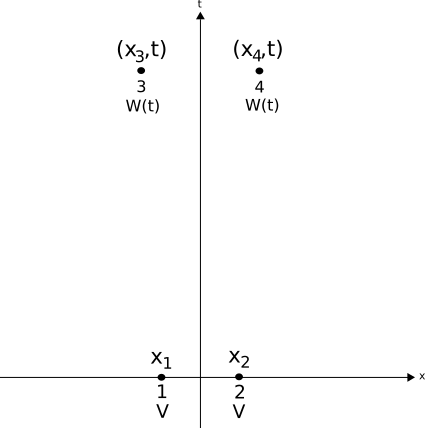
\includegraphics[width=0.41\textwidth]{localops} \caption{\label{fig:localops}The configuration of four pair-wise identical
local operators, themselves separated by large $t$.}
\end{figure}

The spacetime dependence of the conformal blocks appearing in the
4-point function will only depend on the cross-ratio $z=z_{12}z_{34}/z_{13}z_{24}$
(and $\bar{z}$) which is easily shown to be
\[
z=\frac{\sinh\left(\frac{\pi}{\beta}(x_{1}-x_{2})\right)\sinh\left(\frac{\pi}{\beta}(x_{3}-x_{4})\right)}{\sinh\left(\frac{\pi}{\beta}(t-x_{1}+x_{3})\right)\sinh\left(\frac{\pi}{\beta}(t-x_{2}+x_{4})\right)}\,.
\]
As discussed in appendix \ref{sec:Correlators-and-Conformal} we rescale
the 4-point function by the coincident 2-point functions, to scale
out the operator norm. The rescaled correlators then depend only on
the cross-ratios as in \eqref{eq:normcorr}.

As an example, let us consider the identity conformal block in a large
$c$ limit, where the $V$ and $W$ operators have conformal weights
$h_{v}$ and $h_{w}$ respectively. The large $c$ limit is to be
taken with $h_{w}/c$ fixed, and $h_{v}\ll c$ fixed. The conformal
block $\mathcal{F}(z)$ in this limit is computed in \cite{Fitzpatrick:2014vua,Fitzpatrick:2015zha}
\begin{equation}
z^{2h_{v}}\mathcal{F}(z)\approx\left[\frac{z\alpha_{w}(1-z)^{(\alpha_{w}-1)/2}}{1-(1-z)^{\alpha_{w}}}\right]^{2h_{v}}\,,\label{eq:prinblock}
\end{equation}
with $\alpha_{w}=\sqrt{1-24h_{w}/c}$. The real-time out-of-time-order
correlator is obtained by continuing this block to the second Riemann
sheet as described in \cite{PhysRevLett.115.131603} and the leading
contribution to the rescaled commutator is
\begin{equation}
z^{2h_{v}}\mathcal{F}(z)\approx\left[\frac{e^{-\pi i(\alpha_{w}-1)}z\alpha_{w}(1-z)^{(\alpha_{w}-1)/2}}{1-e^{-2\pi i\alpha_{w}}(1-z)^{\alpha_{w}}}\right]^{2h_{v}}\sim\left(\frac{1}{1-\frac{24\pi ih_{w}}{cz}}\right)^{2h_{v}}\,.\label{eq:identityblock}
\end{equation}
Let us take a limit where $\epsilon_{12}=x_{1}-x_{2}$ and $\epsilon_{34}=x_{3}-x_{4}$
are much smaller than $\beta$, and without loss of generality set
$x_{1}=0$. The cross-ratio is then approximately
\[
z\approx\frac{\pi^{2}}{\beta^{2}}\frac{\epsilon_{12}\epsilon_{34}}{\sinh^{2}\left(\frac{\pi}{\beta}\left(t+x_{3}\right)\right)}
\]
provided we stay away from light-like separations where $x_{3}\to-t$.
As we see the conformal block on the second sheet has a simple limit
as $\epsilon_{12}$ and $\epsilon_{34}\to0$, when $z\to0$, corresponding
to the actual computation of the commutator
\begin{equation}
z^{2h_{v}}\mathcal{F}(z)\approx\left(\frac{cz}{24\pi ih_{w}}\right)^{2h_{v}}\,.\label{eq:latetimeblock}
\end{equation}
The exponential decay of this quantity indicates the commutator between
$V$ and $W$ becomes large after a time of order
\begin{equation}
t=\frac{\beta}{4\pi h_{v}}\label{eq:primarytime}
\end{equation}
showing rapid thermalization of primary operators on a timescale much
shorter than \eqref{eq:rstime}.

However the interesting physical question is whether generic states
exhibit some notion of quantum scrambling on a longer timescale. To
explore this question in the current context of CFT 4-point functions,
we can then try to build more generic deformations of the thermal
density matrix by acting with primary operators folded into wavepackets
with some characteristic spatial size $L$. Computing the 4-point
function of these wavepackets, one can attempt to vary $L$ to maximize
the convoluted amplitude, then ask what thermalization timescale emerges.

Concretely, we convolute the function \eqref{eq:identityblock} with
spatial Gaussian wavepackets with width $L$. We will choose $t,L$
and the $x_{i}$ such that light-like singularities in $z$ are avoided.
In this regime, the resulting integral will be dominated by a saddle
point value of $z$, and the convoluted (rescaled) conformal block
may then be well approximated by simply substituting this value into
\eqref{eq:identityblock}. Given the simple form of \eqref{eq:identityblock},
with a cusp at $z=1$, the optimal value for $L$ will be the one
that makes $z$ approach $1$.

For simplicity let us set $x_{1}+x_{2}=x_{3}+x_{4}=0$, and we will
build Gaussian wavepackets in the variables $x_{1}-x_{2}=\ell_{v}$
and $x_{3}-x_{4}=\ell_{w}$. To fix $L$ in terms of $z$, one is
therefore interested in the convolution
\begin{equation}
z(t,L)=\frac{4}{\pi L^{2}}\int_{0}^{\infty}dl_{v}dl_{w}e^{-(l_{v}^{2}+l_{w}^{2})/L^{2}}\frac{\sinh\left(\frac{\pi}{\beta}l_{v}\right)\sinh\left(\frac{\pi}{\beta}l_{w}\right)}{\sinh\left(\frac{\pi}{\beta}\left(t-\frac{l_{v}}{2}+\frac{l_{w}}{2}\right)\right)\sinh\left(\frac{\pi}{\beta}\left(t+\frac{l_{v}}{2}-\frac{l_{w}}{2}\right)\right)}\,.\label{eq:crossratiosmear}
\end{equation}
This formula is justified because the exponential variation of $z$
with $l_{v},l_{w}$ is much more rapid than power law variation of
the conformal block with $z$, so analyzing the convolution of $z$
alone is sufficient to determine $l_{v}$ and $l_{w}$ and subsequently
$L$. The integrand has light-like poles, however for suitable values
of $t$ and $L$ these contributions to the smeared conformal block
can be made negligible. In this limit, the integrand can be well-approximated
by simply
\[
z(t,L)\approx\frac{4}{\pi L^{2}}\int_{0}^{\infty}dl_{v}dl_{w}e^{-(l_{v}^{2}+l_{w}^{2})/L^{2}}\frac{2\sinh\left(\frac{\pi}{\beta}l_{v}\right)\sinh\left(\frac{\pi}{\beta}l_{w}\right)}{\cosh\left(\frac{2\pi}{\beta}t\right)}\,.
\]
This has saddle points when
\[
l_{v}\tanh\left(\frac{l_{v}\pi}{\beta}\right)=\frac{\pi L^{2}}{2\beta}
\]
and likewise for $l_{w}$. The positive solutions are to be taken
corresponding to the limits of integration in \eqref{eq:crossratiosmear}.
If we then ask that the resulting amplitude \eqref{eq:identityblock}
is maximized in magnitude, we find that we must choose $L\sim\beta$
near $t=0$. We choose not to change the shape of the wavepackets
at time increases, and impose this condition for all values of $t$.
At the end we find the optimal value of $z$ is
\begin{equation}
z_{sad}=\mathrm{sech}\left(\frac{2\pi}{\beta}t\right)\label{eq:zsad}
\end{equation}
up to constant factors of order $1$.

Let us now return to the example of the identity conformal block continued
to the second Riemann sheet as considered in \cite{PhysRevLett.115.131603}.
In this case, the saddle point approximation to the (rescaled) convoluted
block function is for sufficiently late times
\begin{equation}
z^{2h_{v}}\mathcal{F}(z)\approx\left(\frac{1}{1-\frac{12\pi ih_{w}}{c}e^{\frac{2\pi}{\beta}(t-x)}}\right)^{2h_{v}}\label{eq:rscorrel}
\end{equation}
where we have restored dependence on the spatial separation $x$ of
the centers of the wavepackets, and inserted the saddle point approximation
value for $z$ \eqref{eq:zsad} for $t\gg\beta$. It is helpful to
plot this for sample parameters as in fig. \ref{fig:scrambling-plot}.
As $t-x$ increases from $0$ to
\begin{equation}
t_{*}=\frac{\beta}{2\pi}\log\frac{c\sqrt{\log2}}{12\pi h_{v}^{1/2}h_{w}}\label{eq:scrambletime}
\end{equation}
the conformal block decreases in magnitude by a factor of about $1/2$.
This thermalization time may be viewed as a proxy for the true scrambling
time of the system, and shows the distinctive appearance of the logarithm
of the system size. The formula is valid for $0<h_{v}\ll c$, but
ideally one would want to argue this formula continues to hold as
$h_{w}$ becomes of order $1$. Unfortunately it is not yet possible
to prove this. We note fig. \ref{fig:scrambling-plot} also shows
in the late-time limit the asymptotic form \eqref{eq:latetimeblock}
is applicable and the timescale for variation is the much shorter
time \eqref{eq:primarytime}.

The correlator of the wavepackets is given by \eqref{eq:rscorrel}
provided one steers clear of the light-cone singularities in \eqref{eq:crossratiosmear}
which render the approximation \eqref{eq:zsad} invalid. This is a
signature that even the wavepackets of primaries are not ideal representatives
of a generic state, and retain regions of spacetime where thermalization
has not yet occurred, outside the light-cone of the wavepacket. Nevertheless
for the present purposes, the reduced state inside the light-cone
appears to be well-thermalized according to the correlators, so this
procedure should yield a good measure of the global scrambling time.
Again it remains to be seen whether \eqref{eq:scrambletime} holds
in the case of most physical interest where $h_{w}$ is of order 1.

\begin{figure}
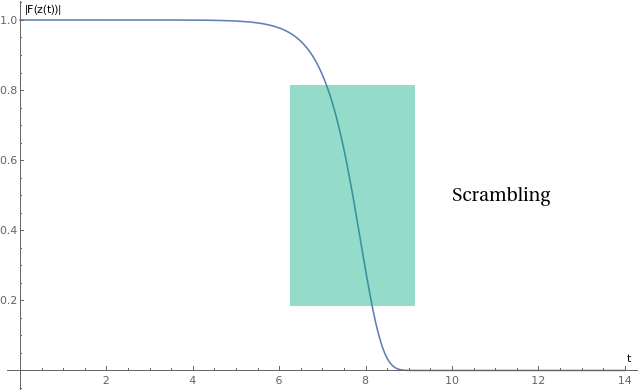
\includegraphics[width=0.45\textwidth]{Fz-t-plot}\qquad{}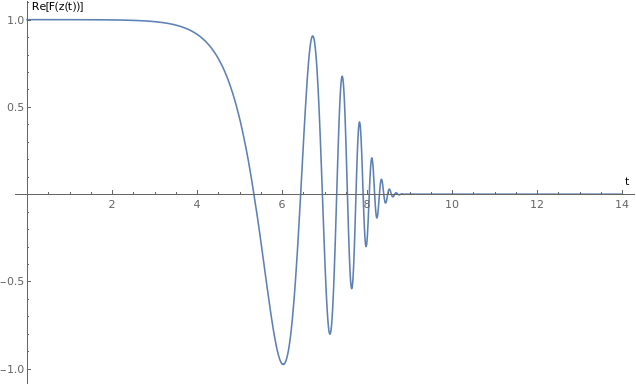
\includegraphics[width=0.45\textwidth]{scrambling-plot-real}
\caption{\label{fig:scrambling-plot}Plot of function $|z^{2h_{v}}\mathcal{F}(z)|=|F(z(t))|=1/\left|1-12\pi ih_{w}\exp\left(2\pi/\beta\left(t-\log c-x\right)\right)\right|^{2h_{v}}$
where $c=10^{7}$, $h_{v}=100$, $h_{w}=10$, $\beta=2\pi$ and $x=0$.
Here $t_{*}=7.7$ according to \eqref{eq:scrambletime}. In the right
panel, a plot of $\mathrm{Re}\,F(z(t))$ is shown.}
\end{figure}

\section{Higher Weight Intermediate States}

We now turn our attention to the contribution of higher weight intermediate
states to the out-of-time order correlators, and will find the surprising
result that these may dominate over the identity block in the late-time
limit. Again we will assume we are taking $c\gg1$ with $h_{w}/c$
fixed and $h_{v}\ll c$ fixed. In addition we will generalize from
the identity block to an intermediate channel with conformal weight
$h_{p}$ fixed as $c\to\infty$.

Our starting point is the formula for the conformal block at next-to-leading
order in this large $c$ expansion of \cite{Fitzpatrick:2015zha}

\[
\mathcal{F}(z)=\mathcal{F}_{0}(z)\left(\frac{1-(1-z)^{\alpha_{w}}}{\alpha_{w}}\right)^{h_{p}}{}_{2}F_{1}\left(h_{p},h_{p},2h_{p},1-(1-z)^{\alpha_{w}}\right)
\]
where $_{2}F_{1}(\alpha,\beta;\gamma;z)$ is the Gauss hypergeometric
function. To continue this expression to the second sheet we use the
hypergeometric function identity \cite{hypergeomexp}
\[
\frac{\Gamma(h)^{2}}{\Gamma(2h)}{}_{2}F_{1}(h,h;2h;w)=\left(\sum_{k=0}^{\infty}\frac{2\left(h\right)_{k}^{2}\left(\psi(k+1)-\psi(h+k)\right)}{k!^{2}}\ensuremath{(1-w)^{k}}\right)-\log(1-w)\,_{2}F_{1}(h,h,1;1-w)
\]
 valid for $|1-w|<1$, where $\left(h\right)_{k}$ is the Pochhammer
symbol, and $\psi(a)$ is the digamma function. Continuing to the
second sheet we then obtain
\begin{align}
\mathcal{F}_{II}(z) & =\mathcal{F}_{0,II}(z)\left(\frac{1-e^{-i2\pi\alpha_{w}}(1-z)^{\alpha_{w}}}{\alpha_{w}}\right)^{h_{p}}\left(_{2}F_{1}\left(h_{p},h_{p},2h_{p},1-e^{-i2\pi\alpha_{w}}(1-z)^{\alpha_{w}}\right)\right.\nonumber \\
+ & \left.2\pi i\alpha_{w}\frac{\Gamma(2h_{p})}{\Gamma(h_{p})^{2}}\,_{2}F_{1}(h_{p},h_{p},1;e^{-i2\pi\alpha_{w}}\left(1-z\right)^{\alpha_{w}})\right)\,.\label{eq:blocktwo}
\end{align}
Expanding for small $h_{w}/c$ and $z\ll1$ leads to
\[
\mathcal{F}_{II}(z)\sim\mathcal{F}_{0,II}(z)\left(\frac{z-\frac{\pi ih_{w}}{6c}}{\alpha_{w}}\right)^{h_{p}}\left(1+i\tan\left(\pi h_{p}\right)-2\pi^{2}iz^{1-2h_{p}}\frac{\Gamma(2h_{p})}{\Gamma(2-2h_{p})\Gamma(h_{p})^{4}\sin\left(2\pi h_{p}\right)}\right)\,.
\]
This ends up being dominated by the last term in the third factor,
and in fact grows at late times. Even at early times ($z$ near 1)
the last term in \eqref{eq:blocktwo} dominates over the other term
in the third factor for $h_{p}>1$. The second factor in \eqref{eq:blocktwo}
rapidly approaches a constant much smaller than 1.

The upshot is the identity block dominates for a finite period of
time, however after
\[
t_{*}\approx\frac{\beta}{4\pi}\log\left(\frac{c}{h_{w}}\right)
\]
the higher weight intermediate states take over. This late time sum
over intermediate states apparently diverges when considered term
by term. This would lead one to conclude the commutator grows initially
while dominated by the identity block, but then may again decrease
at later times, indicating a lack of true scrambling in the conformal
field theory.

One possible way to avoid this conclusion is to demand an infinite
tower of higher weight intermediate primaries, such that the apparently
divergent sum might be resummed to a finite answer. However in the
following section we find contributions for $h_{p}\gg c$ are actually
suppressed. We conclude that even a sparse spectrum of intermediate
primaries with weights $1<h_{p}\ll c$ are sufficient to destroy or
drastically modify the onset of quantum chaos. In light of our previous
discussion, this may simply mean such smeared primaries are still
not good representatives of generic states, and instead one would
need to consider commutators of much more general operators to see
the correct timescale for global thermalization, or quantum scrambling.
Alternatively, it may happen that only operators dual to black hole
states efficiently scramble, and these must be reflected in a choice
of external operators that do not couple at all (or only very weakly)
to higher weight primaries, such that the identity block may dominate
the out-of-time order correlators.

For conformal field theories with holographic anti-de Sitter gravity
duals, the implication of the higher intermediate channels is that
the bulk effective field theory breaks down when it is used to compute
out-of-time-ordered correlators at finite time. On the other hand,
there is no indication of such a breakdown when time-ordered CFT correlators
are computed (see also \cite{Fitzpatrick:2016ive,Fitzpatrick:2016mjq}),
which correspond to the boundary $S$-matrix of the bulk theory. To
see this we simply note that as higher dimensional operators in CFT$_{2}$
correspond to interactions of increasing mass scale in AdS$_{3}$,
domination of all intermediate channels with dimension $h_{p}\geq1$
means that there would be a dual set of an infinite sequence of interactions
in the gravitation theory in AdS$_{3}$. If these high scale interactions
affect the infrared physics of the theory, then the standard decoupling
theorems of effective field theory such \cite{PhysRevD.11.2856}
break down.

Now the usual measurements we perform can be well-approximated by
transition amplitudes, built out of time-ordered correlators which
may be computed as within effective field theory. It is only the particular
set of observables corresponding to out-of-time-order correlators,
or norms of commutators that exhibit this peculiar behavior. For the
black hole information problem this would seem to imply that contrary
to expectations, commutators that measure limits on the causal propagation
of information are indeed observables sensitive to the ultra-violet
structure of the theory, as long hinted at in perturbative string
theory computations \cite{Lowe:1995pu,Lowe:1995ac}.

\section{Intermediate Channels with $h_{p}\gg c$}

So far we have only considered intermediate channels with fixed $h_{p}\ll c$.
It is also instructive to perform the same analysis for intermediate
channels with $h_{p}\gg c$ where the limit is $h_{p}\to\infty$ with
$c/h_{p}$, $h_{v}/h_{p}$ and $h_{w}/h_{p}$ fixed and small. For
this we consider equation (16) in \cite{Zam87},
\begin{equation}
\mathcal{F}(z)=\left(16q\right)^{h_{p}-\frac{c}{24}}z^{\frac{c}{24}-2h_{v}}(1-z)^{\frac{c}{24}-(h_{v}+h_{w})}\theta_{3}(q)^{\frac{c}{2}-8(h_{v}+h_{w})}H(c,h_{p},h_{i},q)\label{eq:eq16zem87}
\end{equation}
where the nome $q=e^{i\pi\tau}$ is related to the cross-ratio $z$
by
\[
\tau=i\frac{K'(z)}{K(z)}=i\frac{K(1-z)}{K(z)}
\]
where $K(z)$ is the complete elliptic integral with parameter\footnote{We clarify that in most mathematical literature, the complete elliptic
integral $K$ is defined with the modulus $k$ as the argument. Our
$z$ is related to $k$ through $z=k^{2}$. It is also common for
many mathematicians to use the symbol $m$ for our $z$.} $z$. Here $H$ is a function that is $1+O(1/h_{p})$ and
\begin{equation}
\theta_{3}(q)=\sum_{n=-\infty}^{\infty}q^{n^{2}}\,.\label{eq:thetathree}
\end{equation}

Eq.~(\ref{eq:eq16zem87}) has a branch cut at $z=1$ from the $1-z$
factor which will lead to the same analytic behavior for the intermediate
case $h_{p}\ll c$, which we have previously considered. To see this
we expand the nome $q$ around $z=0$ to obtain
\[
q=e^{i\pi\tau}=\frac{z}{16}+\frac{z^{2}}{32}+\cdots\,.
\]
As $\theta_{3}(q)$ is regular near $q=0$, we see that on the principal
sheet $\mathcal{F}(z)$ goes to zero as $z\to0$. Therefore the heavy
intermediate channels are perfectly suppressed on the first Riemann
sheet. Crossing the branch cut $z=1$ from above, the complete elliptic
function $K(z)$ picks up an additional imaginary part \cite{Bogner:2017vim}:
\[
\lim_{\epsilon\to0^{+}}K(z+i\epsilon)=K(z)+2iK(1-z)\,.
\]
Analyticity implies that on the second Riemann sheet the nome is now
\[
q=\exp\left[-\frac{\pi K(1-z)}{K(z)+2iK(1-z)}\right]=\exp\left[-\frac{\pi}{\frac{K(z)}{K(1-z)}+2i}\right]\,.
\]
To expand this expression near $z=0$, we use
\[
\frac{K(z)}{K(1-z)}\approx\frac{\pi}{4\log2-\log z}+\mathcal{O}\left(\frac{z}{\log^{2}z}\right)
\]
so that
\begin{equation}
q\approx e^{\frac{i\pi}{2}+\frac{\pi^{2}}{4\log z}}\,.\label{eq:nomeexpan}
\end{equation}
We then need to expand \eqref{eq:thetathree} near $q=i$. The expansion
near $q=1$ is
\[
\left|\theta_{3}(q)\right|\approx\left|\frac{\sqrt{\pi}}{\sqrt{1-q}}\right|
\]
but we can obtain the expansion near $q=i$ by using the relation
\[
\left|\theta_{3}(q)\right|=\left|\frac{\sqrt{\pi}}{\sqrt{\log q}}\theta_{3}\left(e^{\frac{\pi^{2}}{\log q}}\right)\right|
\]
and substituting in \eqref{eq:nomeexpan} to give $\theta_{3}(q)$
near $q=i$ as
\begin{equation}
\left|\theta_{3}(q)\right|\approx\left|\frac{\sqrt{-2\log z}}{\sqrt{\pi}}\right|\,.\label{eq:nomeneari}
\end{equation}
Assembling the various factors, we find again a dramatic enhancement
of the higher weight channel on the second Riemann sheet arising from
the behavior \eqref{eq:nomeneari}, compared to the behavior on the
principal sheet. However when we compare to the $h_{p}=0$ expression
of the previous section, the $z^{c/24}$ factor of \eqref{eq:eq16zem87}
dominates for small $z$ so we conclude they do not dominate versus
the identity channel (again modulo restrictions on the operator couplings
$C_{p}$ of \eqref{eq:blockdef}).

\section{Conclusions}

In this chapter we discussed the issue of smearing local operators in
a thermal CFT and its connection with quantum scrambling. We pointed
out that the correct scrambling time should be identified with operators
that maximize the timescale of variation of the out-of-time ordered
correlator, which may occur well before the asymptotic late-time limit.
We then examined a somewhat independent issue, that the higher intermediate
states with $0<h_{p}\ll c$ can have large out-of-time ordered correlators.
We discussed the implications of this statement, which is that in
the AdS$_{3}$ gravity dual the UV dynamics and IR dynamics is no
longer decoupled when these observables are computed. This lack of
decoupling appears even when the usual time-ordered correlators, or
transition amplitudes satisfy the standard decoupling lore. When applied
to scattering in $AdS_{3}$ black hole backgrounds this implies that
the commutators that lead one to conclude information is lost semiclassically,
are in fact not computable without a full specification of the ultraviolet
physics of the theory. The ordinary bulk effective field theory does
not predict its own demise when computing these observables.

As for the appearance of a scrambling time of the form \eqref{eq:rstime}
we have found a variant of this expression \eqref{eq:scrambletime},
valid when the identity block dominates. The expression involves a
term of the form $\beta/2\pi\log c$, but other significant terms
are also present. If other intermediate primaries appear, with conformal
weights fixed in a large $c$ limit, they will dominate the late-time
behavior and may completely spoil thermalization. It will be very
interesting to extend the range of validity of these expressions to
determine whether there exist a class of 2d conformal field theories
that may be viewed as fast scramblers at finite temperature.


\chapter{Holographic Map for Cosmological Horizons}\label{chap:map}
We propose a holographic map between Einstein gravity coupled to matter
in a de Sitter background and large $N$ quantum mechanics of a system
of spins. Holography maps a spin model with a finite dimensional Hilbert
space defined on a version of the stretched horizon into bulk gravitational
dynamics. The full Hamiltonian of the spin model contains a non-local
piece which generates chaotic dynamics, widely conjectured to be a
necessary part of quantum gravity, and a local piece which recovers
the perturbative spectrum in the bulk.

\section{Introduction}

Previous work has argued for a unitary, holographic description of
black hole dynamics via certain spin models \cite{Lowe:2016mhi,Lowe:2017ehz}
defined on the stretched horizon \cite{thorne1986black} of the black
hole. These spin models have the common feature that non-local interactions
generate chaotic dynamics, widely conjectured to be an integral part
of a full quantum mechanical description of gravity \cite{Sekino:2008he}.
In this chapter we argue that a similar approach works for the cosmological
horizon in de Sitter spacetime, given that the static patch metric
has a similar form to the metric in Schwarzschild coordinates. To
this end we will give an explicit prescription to map perturbative
bulk fields to a quantum mechanical operator defined in the holographic
spin model. This map will then allow us to construct a local Hamiltonian
that reproduces the classical energy of a perturbation around de Sitter
spacetime. We argue that this local Hamiltonian, together with the
non-local long-range interaction necessary to generate chaotic dynamics,
can potentially be a viable description of de Sitter quantum gravity.

Before we begin, we will review relevant facts of the de Sitter space-time
to establish our convention of notations. We mostly follow the conventions
in Ref.~\cite{Spradlin:2001pw}. Throughout the chapter we will restrict
our discussion to $(1+3)$-dimensional space-time entirely, although
the methodology presented can in principle be applied to higher (or
lower) dimensions. Our metric signatures are always mostly positive,
i.e.~$(-++\cdots)$.

Static coordinates cover only one triangular region in the Penrose
diagram (see Fig.~\ref{penrose})
\begin{equation}
\dd s^{2}=-(1-\frac{r^{2}}{\ell^{2}})\,\dd t^{2}+\frac{\dd r^{2}}{1-\frac{r^{2}}{\ell^{2}}}+r^{2}\,\dd\Omega^{2}\label{eq:static}
\end{equation}
where $\dd\Omega^{2}=\dd\theta^{2}+\sin^{2}\theta\,\dd\varphi^{2}$
is the line element on the unit 2-sphere $S^{2}$ and $\ell$ is the
radius of curvature of the de Sitter spacetime.

\begin{figure}\centering
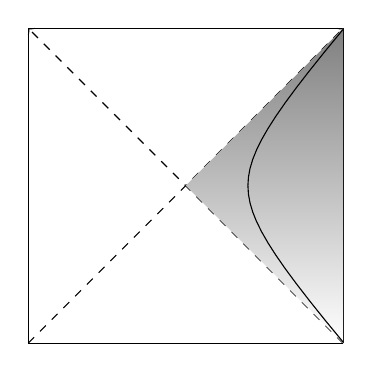
\begin{tikzpicture}[scale=1]
    \draw (-2,2) -- (2,2);
    \draw (-2,2) -- (-2,-2);
    \draw (-2,-2) -- (2,-2);
    \draw (2,-2) -- (2,2);
    \draw[->,dashed] (-2,-2) -- (2,2);
    \draw[->,dashed] (2,-2) -- (-2,2);
    \shade (0,0) -- (2,2) -- (2,-2) -- (0,0);
    \pgfmathsetmacro{\e}{1.5}   % eccentricity
    \pgfmathsetmacro{\a}{0.7}
    \pgfmathsetmacro{\b}{(\a*sqrt((\e)^2-1)}
    \draw plot[domain=-1.66:1.66] ({\a*cosh(\x)+0.09},{\b*sinh(\x)});
  \end{tikzpicture} \caption{Penrose diagram for de-Sitter spacetime, where shaded region is covered
by the static coordinates. The stretched horizon (solid curve inside
the static patch) is defined as a hypersurface at fixed $r$.}
\label{penrose}
\end{figure}


\section{Mode Functions in de-Sitter}

\subsection{Static Patch}

Our goal is to construct a spin model which reproduces the bulk spectrum
in a de Sitter background. To proceed we first review some standard
results concerning mode functions in static de Sitter. For simplicity,
we will treat the massless minimally coupled scalar, and follow the
point of view of \cite{Danielsson:2002qh} that with a cutoff to
exclude the zero mode, the system can be quantized around the Bunch-Davies
(or Euclidean) vacuum state. Had we been interested in the system
including the zero-mode, this quantization preserving de Sitter isometries
would be inadmissible \cite{Allen:1987tz}. This quantization of
the massless minimally coupled scalar around the Bunch-Davies vacuum
is closely related to that of perturbative gravitons, as explained
in \cite{Bernar:2016zgq,Bernar:2018nww}. The results may then be
straightforwardly applied to other bulk modes once this case is understood.

We begin by considering modes in the static patch \eqref{eq:static}.
The equation of motion for the free scalar field $\Phi(t,r,\theta,\phi)$
is
\[
\frac{\partial_{t}^{2}\Phi}{1-r^{2}/\ell^{2}}-\frac{\partial_{r}[r^{2}(1-r^{2}/\ell^{2})\partial_{r}\Phi]}{r^{2}}-\frac{\partial_{\theta}(\sin\theta\partial_{\theta}\Phi)}{r^{2}\sin\theta}-\frac{\partial_{\varphi}^{2}\Phi}{r^{2}\sin^{2}\theta}=0\,.
\]
Separating variables, we have
\[
\Phi_{\omega lm}(t,r,\theta,\varphi)=A_{\omega l}e^{-i\omega t}f_{\omega l}(r)Y_{lm}(\theta,\varphi)\,,
\]
where $f_{\omega l}(r)$ satisfies
\[
(1-r^{2}/\ell^{2})f''_{\omega l}(r)+\frac{2(1-2r^{2}/\ell^{2})}{r}f'_{\omega l}(r)+\left(\frac{\omega^{2}}{1-r^{2}/\ell^{2}}-\frac{l(l+1)}{r^{2}}\right)f_{\omega l}(r)=0\,.
\]
We pick the set of solutions that are regular at $r=0$ and find
\[
f_{\omega l}(r)=\frac{(r/\ell)^{l}}{\ell}(1-r^{2}/\ell^{2})^{i\omega\ell/2}{}_{2}{\rm F}_{1}\left(\frac{l+i\omega\ell}{2},\frac{l+i\omega\ell+3}{2};l+\frac{3}{2};\frac{r^{2}}{\ell^{2}}\right)\,.
\]
We fix the normalization constant $A_{\omega l}$ by computing the
Klein-Gordon norm. This is defined on a spacelike surface $\Sigma$
by
\begin{align*}
\left\langle f,g\right\rangle  & =-i\int_{\Sigma}\dd\Sigma\,n^{\lambda}\,(f\partial_{\lambda}g^{*}-g^{*}\partial_{\lambda}f)
\end{align*}
where $n^{\lambda}$ is a timelike unit vector normal to $\Sigma$.
Evaluating this on a constant $t$ slice gives
\begin{equation}
\left\langle f,g\right\rangle =-i\int(f\partial_{t}g^{\star}-g^{\star}\partial_{t}f)\frac{r^{2}\,\dd r\,\sin\theta\,\dd\theta\,\dd\varphi}{1-r^{2}/\ell^{2}}\,.\label{eq:innerprod}
\end{equation}
Computing the mode normalization then gives
\[
\left\langle \Phi_{\omega lm},\Phi_{\omega'l'm'}\right\rangle =A_{\omega l}A_{\omega'l}^{\star}(\omega+\omega')\delta_{ll'}\delta_{mm'}\int_{0}^{\ell}\frac{f_{\omega l}(r)f_{\omega'l}^{\star}(r)\,r^{2}\,\dd r}{1-r^{2}/\ell^{2}}\,.
\]
Using the equation of motion for $f_{\omega l}(r)$ we have
\[
[r^{2}(1-r^{2}/\ell^{2})f'_{\omega l}(r)]'\,f_{\omega'l}^{\star}(r)+\left(\frac{\omega^{2}r^{2}}{1-r^{2}/\ell^{2}}-l(l+1)\right)f_{\omega l}(r)f_{\omega'l}^{\star}(r)=0
\]
and likewise
\[
[r^{2}(1-r^{2}/\ell^{2})f_{\omega'l}^{\star\prime}(r)]'\,f_{\omega l}(r)+\left(\frac{\omega'^{2}r^{2}}{1-r^{2}/\ell^{2}}-l(l+1)\right)f_{\omega'l}^{\star}(r)f_{\omega l}(r)=0\,.
\]
Subtracting we have
\[
\frac{(\omega^{2}-\omega'^{2})r^{2}}{1-r^{2}/\ell^{2}}f_{\omega l}(r)f_{\omega'l}^{\star}(r)=[r^{2}(1-r^{2}/\ell^{2})f_{\omega'l}^{\star\prime}(r)]'\,f_{\omega l}(r)-[r^{2}(1-r^{2}/\ell^{2})f'_{\omega l}(r)]'\,f_{\omega'l}^{\star}(r)\,,
\]
and integrating by parts, we have
\[
\int_{0}^{\ell}\frac{(\omega^{2}-\omega'^{2})r^{2}}{1-r^{2}/\ell^{2}}f_{\omega l}(r)f_{\omega'l}^{\star}(r)=r^{2}(1-r^{2}/\ell^{2})f_{\omega'l}^{\star\prime}(r)\,f_{\omega l}(r)-r^{2}(1-r^{2}/\ell^{2})f'_{\omega l}(r)\,f_{\omega'l}^{\star}(r)\Big|_{0}^{\ell}\,.
\]
This gives
\[
\int_{0}^{\ell}\frac{r^{2}\,\dd r}{1-r^{2}/\ell^{2}}f_{\omega l}(r)f_{\omega'l}^{\star}(r)=\frac{\ell^{2}}{\omega^{2}-\omega'^{2}}\lim_{r\to\ell}\,(1-r^{2}/\ell^{2})\left[f_{\omega'l}^{\star\prime}(r)\,f_{\omega l}(r)-f'_{\omega l}(r)\,f_{\omega'l}^{\star}(r)\right]\,.
\]
Using the hypergeometric identity near $z=1$
\[
_{2}{\rm F}_{1}(a,b,c,z)=\frac{\Gamma(c)\Gamma(c-a-b)}{\Gamma(c-a)\Gamma(c-b)}+\frac{\Gamma(c)\Gamma(a+b-c)}{\Gamma(a)\Gamma(b)}(1-z)^{c-a-b}
\]
we can expand $f_{\omega l}(r)$ near $r=\ell$ to give
\[
\ell f_{\omega l}(r)\approx\frac{\Gamma(l+\frac{3}{2})\Gamma(-i\ell\omega)}{\Gamma\left(\frac{l-i\omega\ell}{2}\right)\Gamma\left(\frac{l-i\omega l+3}{2}\right)}(1-r^{2}/\ell^{2})^{\frac{i\ell\omega}{2}}+\frac{\Gamma(l+\frac{3}{2})\Gamma(i\ell\omega)}{\Gamma\left(\frac{l+i\omega\ell}{2}\right)\Gamma\left(\frac{l+i\omega l+3}{2}\right)}(1-r^{2}/\ell^{2})^{-\frac{i\ell\omega}{2}}\,.
\]
Letting
\[
B_{\omega l}=\frac{\Gamma(l+\frac{3}{2})\Gamma(i\ell\omega)}{\Gamma\left(\frac{l+i\omega\ell}{2}\right)\Gamma\left(\frac{l+i\omega l+3}{2}\right)}
\]
we see that we have
\[
\ell f_{\omega l}(r)\approx B_{\omega l}^{\star}(1-r^{2}/\ell^{2})^{\frac{i\ell\omega}{2}}+B_{\omega l}(1-r^{2}/\ell^{2})^{-\frac{i\ell\omega}{2}}
\]
and
\[
f'_{\omega l}(r)\approx\frac{-i\omega}{1-r^{2}/\ell^{2}}\left[B_{\omega l}^{\star}(1-r^{2}/\ell^{2})^{\frac{i\ell\omega}{2}}-B_{\omega l}(1-r^{2}/\ell^{2})^{-\frac{i\ell\omega}{2}}\right]\,.
\]
Multiplying $f_{\omega l}(r)$ and $f'_{\omega l}(r)$ and dropping
terms that are rapidly oscillating as $|\omega-\omega'|>0$ and $r\to\ell$,
we find that
\begin{equation}
\int_{0}^{\ell}\frac{r^{2}\,\dd r}{1-r^{2}/\ell^{2}}f_{\omega l}(r)f_{\omega'l}^{\star}(r)=\lim_{r\to\ell}\frac{2|B_{\omega l}|^{2}}{\omega-\omega'}\sin\left[\frac{\left(\omega-\omega'\right)\ell}{2}\log\left(\frac{1}{1-r^{2}/\ell^{2}}\right)\right]\label{eq:radialint}
\end{equation}
Using
\[
\lim_{C\to\infty}\frac{\sin Cx}{x}=\pi\delta(x)
\]
we have
\[
\int_{0}^{\ell}\frac{r^{2}\,\dd r}{1-r^{2}/\ell^{2}}f_{\omega l}(r)f_{\omega'l}^{\star}(r)=2\pi|B_{\omega l}|^{2}\delta(\omega-\omega')
\]
or
\begin{equation}
\left\langle \Phi_{\omega lm},\Phi_{\omega'l'm'}\right\rangle =4\pi|A_{\omega l}|^{2}|B_{\omega l}|^{2}\delta_{ll'}\delta_{mm'}\omega\delta(\omega-\omega')\,.\label{eq:staticnorm}
\end{equation}
If we normalize according to
\[
\left\langle \Phi_{\omega lm},\Phi_{\omega'l'm'}\right\rangle =\delta_{ll'}\delta_{mm'}\omega\delta(\omega-\omega')\,,
\]
we need to pick $A_{\omega l}$ such that
\[
|A_{\omega l}|^{2}=\frac{1}{4\pi|B_{\omega l}|^{2}}\,.
\]


\subsection{Flat Slicing}

Now let us consider the analogous problem for modes in the flat slicing.
The metric takes the form
\[
\dd s^{2}=-\dd\tau^{2}+e^{2\tau/\ell}\dd\vec{x}^{2}=-\dd\tau^{2}+e^{2\tau/\ell}(\dd\rho^{2}+\rho^{2}\dd\theta^{2}+\rho^{2}\sin^{2}\theta\dd\varphi^{2})
\]
where $\tau\in(-\infty,+\infty)$ and $\rho\in(0,+\infty)$. The wave
equation for the massless minimally coupled scalar is given by
\[
\partial_{\tau}^{2}\phi+\frac{3}{\ell}\partial_{\tau}\phi-e^{-2\tau/\ell}\Delta\phi=0
\]
where $\Delta\phi$ is the usual spatial Laplacian operator
\[
\Delta\phi=\partial_{\rho}^{2}\phi+\frac{2}{\rho}\partial_{\rho}\phi+\frac{\partial_{\theta}^{2}\phi}{\rho^{2}}+\frac{\partial_{\theta}\phi}{\rho^{2}\tan\theta}+\frac{\partial_{\varphi}^{2}\phi}{\rho^{2}\sin^{2}\theta}\,.
\]
Separating variables, we use the ansatz
\[
\phi_{klm}(\tau,\rho,\theta,\varphi)=T_{k}(\tau)R_{kl}(\rho)Y_{lm}(\theta,\varphi)
\]
where $T_{k}(\tau)$ satisfies
\[
T''(\tau)+\frac{3}{\ell}T'(\tau)+k^{2}e^{-2\tau/\ell}T(\tau)=0
\]
and $R_{kl}(\rho)$ satisfies
\[
R''(\rho)+\frac{2}{\rho}R'(\rho)+\left(k^{2}-\frac{l(l+1)}{\rho^{2}}\right)R(\rho)=0\,.
\]
Assuming regularity at $\rho=0$ we can solve for $R(\rho)$
\[
R_{kl}(\rho)=C_{kl}\,j_{l}(k\rho)
\]
where $j_{l}(x)$ is the spherical Bessel function of first kind $j_{l}(x)=\sqrt{\frac{\pi}{2x}}J_{l+\frac{1}{2}}(x)$.
We will determine the normalization constant $C_{kl}$ later.

The equation for $T(\tau)$ can be solved to give
\[
T_{k}(\tau)=c_{1}e^{ik\ell e^{-\tau/\ell}}\left(1-ik\ell e^{-\tau/\ell}\right)+c_{2}e^{-ik\ell e^{-\tau/\ell}}\left(1+ik\ell e^{-\tau/\ell}\right)
\]
or, in terms of the conformal time $\eta=-\ell e^{-\tau/\ell}$
\[
T_{k}(\tau)=c_{1}e^{-ik\eta}\left(1+ik\eta\right)+c_{2}e^{ik\eta}\left(1-ik\eta\right)\,.
\]
We assume Bunch-Davies vacuum and therefore pick the special solution
\[
T_{k}(\eta)=e^{-ik\eta}\left(1+ik\eta\right)
\]
and absorb the normalization constant into $C_{kl}$, which we will
fix now. The mode functions are normalized according to the Klein-Gordon
norm
\[
\left\langle f,g\right\rangle =-i\int_{\Sigma}(f\partial_{\mu}g^{\star}-g^{\star}\partial_{\mu}f)\,n^{\mu}\sqrt{\gamma}\,\dd^{3}x\,.
\]
Here $\Sigma$ is a spacelike hypersurface with unit norm $n^{\mu}$
and $\sqrt{\gamma}$ is the spatial volume element. We pick the $\tau=0$
timeslice in the flat slicing since the metric at $\tau=0$ is conveniently
the Minkowski metric. In addition, we have $\partial_{\tau}=\partial_{\eta}$
on the $\tau=0$ timeslice. We therefore have
\[
\left\langle f,g\right\rangle =-i\int(f\partial_{\tau}g^{\star}-g^{\star}\partial_{\tau}f)\,\rho^{2}\,\dd\rho\,\sin\theta\,\dd\theta\,\dd\varphi\,.
\]
We use this to fix the normalization factor $C_{kl}$. We have, for
the $\phi_{klm}$ modes on $\tau=0$
\[
\partial_{\tau}\phi_{klm}=-C_{kl}\,k^{2}\ell\,e^{ik\ell}j_{l}(k\rho)\,Y_{lm}(\theta,\varphi)\,.
\]
Therefore
\[
\left\langle \phi_{klm},\phi_{k'l'm'}\right\rangle =i\ell C_{kl}C_{k'l'}^{\star}\,\delta_{ll'}\delta_{mm'}e^{i(k-k')\ell}\int[(1-ik\ell)k'^{2}-(1+ik'\ell)k^{2}]j_{l}(k\rho)j_{l}(k'\rho)\rho^{2}\,\dd\rho\,.
\]
Using the orthogonality of spherical Bessel functions
\[
\int_{0}^{\infty}\rho^{2}j_{l}(u\rho)j_{l}(v\rho)\,\dd\rho=\frac{\pi}{2u^{2}}\delta(u-v)
\]
we have
\[
\left\langle \phi_{klm},\phi_{k'l'm'}\right\rangle =\ell^{3}\,\pi k\,|C_{kl}|^{2}\,\delta_{ll'}\delta_{mm'}\delta(k\ell-k'\ell)\,.
\]
We therefore find
\[
C_{kl}=\frac{1}{\sqrt{\pi k\ell}}\frac{1}{\ell}\,,
\]
and the full solution is therefore
\[
\phi_{klm}(\tau,\rho,\theta,\varphi)=\frac{1}{\ell\sqrt{\pi k\ell}}\,e^{-ik\eta}(1+ik\eta)\,j_{l}(k\rho)\,Y_{lm}(\theta,\varphi)\,.
\]


\subsection{Matching Modes Across the Cosmological Horizon}

\begin{figure}
\centering
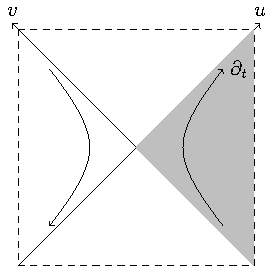
\includegraphics{penrose}\caption{\label{fig:Penrose-diagram-for}Penrose diagram for the de-Sitter spacetime. Flat
slicing modes cover the right upper half of the diagram and are matched
to static patch modes on the line $u=0$. Positive frequency modes
in the Bunch-Davies vacuum are then analytic in the lower-half-complex
$v-$plane.}

\end{figure}

Following \cite{PhysRevD.14.870}, modes in the flat slicing may be viewed
as modes entangled across the left and right static patches. In Kruskal
coordinates in the right static patch $u=e^{x^{-}/\ell}$ and $v=-e^{-x^{+}/\ell}$
(other choices of sign generate the other patches in static coordinates)
where $x^{\pm}=t\pm r^{\star}$ and
\[
r^{\star}=\frac{\ell}{2}\log\frac{1+r/\ell}{1-r/\ell}\approx\frac{\ell}{2}\log\frac{2}{1-r/\ell}
\]
we have
\[
\Phi_{\omega lm}\approx A_{\omega l}(B_{\omega l}^{\star}2^{i\omega\ell}|v|^{i\omega\ell}+B_{\omega l}2^{-i\omega\ell}|u|^{-i\omega\ell})Y_{lm}(\theta,\varphi)
\]
 near the cosmological horizon.

We now define a mode function $\Phi_{\omega lm}^{+}$ which is non-zero
on the right quadrant, and a $\Phi_{\omega lm}^{-}$ which is non-zero
on the left quadrant. We require that the linear combination
\[
\bar{\Phi}_{\omega lm}=c\,\Phi_{\omega lm}^{+}+d\,\Phi_{\omega lm}^{-}
\]
be analytic in the lower half $v-$plane on the past horizon on the
right (and the past horizon on the left), i.e. the surface $u=0$.
On the right quadrant we can rewrite the function $(-v)^{i\omega\ell}=(e^{i\pi}v)^{i\omega\ell}=e^{-\pi\omega\ell}v^{i\omega\ell}$.
Therefore, the linear combination $\Phi_{\omega lm}^{+}+e^{-\pi\omega\ell}\Phi_{\omega lm}^{-}$
is analytic in the lower-half-complex $v-$plane at $u=0$ (see fig.
\ref{fig:Penrose-diagram-for}) corresponding to a combination of
positive frequency flat-slicing modes. The properly normalized mode
is
\begin{equation}
\bar{\Phi}_{\omega lm}=\frac{1}{\sqrt{2\sinh(\pi\omega\ell)}}\left(e^{\pi\omega\ell/2}\Phi_{\omega lm}^{+}+e^{-\pi\omega\ell/2}\Phi_{\omega lm}^{-}\right)\,.\label{eq:entmode}
\end{equation}
This mode is analytic in the lower-half $v$-plane for either choice
of sign for $\omega$, so should be identified with a linear combination
of positive $k$ flat-slicing modes.

We can now expand a quantum field operator $\hat{\Phi}$ in terms
of normal modes
\begin{align*}
\hat{\Phi} & =\int_{0}^{\infty}dk\sum_{lm}\phi_{klm}a_{klm}+{\rm h.c.\,(flat\,slicing)}\\
 & =\int_{0}^{\infty}d\omega\sum_{lm}\Phi_{\omega lm}^{+}b_{\omega lm}^{+}+\Phi_{\omega lm}^{{\rm -}}b_{\omega lm}^{{\rm -}\dagger}+{\rm h.c.\,(static\,patches)}\\
 & =\int_{-\infty}^{\infty}d\omega\sum_{lm}\bar{\Phi}_{\omega lm}c_{\omega lm}+{\rm h.c.\,(entangled\,static\,patches)}\,.
\end{align*}
We define the Bunch-Davies vacuum $|0\rangle$ to be annihilated by
all $a_{klm}$ with $k>0$
\[
a_{klm}|0\rangle=0
\]
which coincides with
\[
c_{\omega lm}\left|0\right\rangle =0
\]
for $-\infty<\omega<\infty$. We similarly define the static patch
vacuum $|\Omega\rangle$ to be annihilated by all $b_{\omega lm}^{\pm}$
with $\omega>0$
\[
b_{\omega lm}^{\pm}|\Omega\rangle=0\,.
\]
From the relation we obtained between $\Phi^{\pm}$ and $\bar{\Phi}$
we obtain the relations between $b_{\omega lm}^{\pm}$ and $c_{\omega lm}$
\begin{align*}
c_{\omega lm} & =\begin{cases}
\frac{1}{\sqrt{2\sinh{\pi\omega\ell}}}\left(e^{\pi\omega\ell/2}b_{\omega lm}^{+}+e^{-\pi\omega\ell/2}b_{\omega lm}^{-\dagger}\right) & \omega>0\\
\frac{1}{\sqrt{2\sinh{\pi\omega\ell}}}\left(e^{\pi\omega\ell/2}b_{\omega lm}^{+\dagger}+e^{-\pi\omega\ell/2}b_{\omega lm}^{-}\right) & \omega<0\,.
\end{cases}
\end{align*}
As usual, the vacuum state $\left|0\right\rangle $ becomes a thermal
density matrix in the right static patch when the modes $b_{\omega lm}^{-}$
are traced over.

We now need to compute the overlap of modes $\Phi_{\omega lm}$ with
$\phi_{\omega lm}$ to construct the Bogoliubov transformation. In
order to perform the integrals, we need the coordinate transformation
between $(t,r)$ and $(\eta,\rho)$. We define null coordinates in
the flat slicing
\[
U=\frac{\eta-\rho}{2}\qquad V=\frac{\eta+\rho}{2}
\]
leading to the metric. In the flat slicing using the $(\eta,\rho)$
coordinates the metric is
\[
\dd s^{2}=\frac{\ell^{2}}{\eta^{2}}(-\dd\eta^{2}+\dd\rho^{2}+\rho^{2}\dd\Omega^{2})
\]
which in terms of $(U,V)$ coordinates becomes
\[
\dd s^{2}=\frac{\ell^{2}}{(U+V)^{2}}(-4\dd U\dd V+(V-U)^{2}\dd\Omega^{2})\,.
\]
In the static patch, we define null coordinates $(u,v)$
\[
u=e^{x^{-}/\ell}\,,v=-e^{-x^{+}/\ell}
\]
and one verifies that the metric is
\[
\dd s^{2}=\frac{\ell^{2}}{(1-uv)^{2}}(-4\dd u\dd v+(1+uv)^{2}\dd\Omega^{2})\,.
\]
We see that the relation between $(u,v)$ and $(U,V)$ is simply
\[
U=-\frac{\ell}{u}\qquad V=\ell v
\]
which gives
\[
\eta=-\frac{\ell}{u}+\ell v\qquad\rho=\frac{\ell}{u}+\ell v\,.
\]
The flat slicing mode function therefore becomes
\[
\phi_{klm}=\frac{1}{\ell}\frac{1}{\sqrt{\pi k\ell}}\,e^{ik\ell(\frac{1}{u}-v)}\left[1-ik\ell\left(\frac{1}{u}-v\right)\right]\,\frac{\sin(k\ell(v+1/u)-l\pi/2)}{k\ell(v+1/u)}\,Y_{lm}(\theta,\varphi)
\]
where we have used the behavior of spherical Bessel function at infinity
\[
\lim_{\rho\to\infty}j_{l}(k\rho)=\frac{\sin(k\rho-l\pi/2)}{k\rho}\,.
\]
Near the past horizon on the left patch, $u\to0$ with $v$ fixed,
the flat slice mode becomes
\[
\phi_{klm}=\frac{1}{\ell}\frac{-i}{\sqrt{\pi k\ell}}\,e^{ik\ell(\frac{1}{u}-v)}\sin(k\ell(v+1/u)-l\pi/2)\,Y_{lm}(\theta,\varphi)\,.
\]
Using the identity $\sin z=(e^{iz}-e^{-iz})/2i$ we can rewrite the
flat slice mode function as
\begin{align*}
\phi_{klm} & =\frac{1}{\ell}\frac{-1}{2\sqrt{\pi k\ell}}\,e^{ik\ell(\frac{1}{u}-v)}(i^{-l}e^{ik\ell(v+1/u)}-i^{l}e^{-ik\ell(v+1/u)})Y_{lm}(\theta,\varphi)\\
 & =\frac{1}{\ell}\frac{1}{2\sqrt{\pi k\ell}}(i^{l}e^{-2ik\ell v}-i^{-l}e^{2ik\ell/u})Y_{lm}(\theta,\varphi)\sim\frac{1}{\ell}\frac{i^{l}}{2\sqrt{\pi k\ell}}e^{-2ik\ell v}Y_{lm}(\theta,\varphi)\,.
\end{align*}
We have shown above that near the past horizon the static patch mode
is
\[
\Phi_{\omega lm}=A_{\omega l}B_{\omega l}^{\star}(-v)^{i\omega\ell}2^{i\omega\ell}Y_{lm}(\theta,\varphi)\,.
\]
On the past horizon the Klein-Gordon norm is
\[
\left\langle f,g\right\rangle =-i\ell^{2}\int\dd\Omega\dd v\,(f\partial_{v}g^{\star}-g^{\star}\partial_{v}f)=i\ell^{2}\int_{-\infty}^{0}\dd\Omega\left(2\int g^{\star}\partial_{v}f\,\dd v-g^{\star}f\Big|_{0}^{-\infty}\right)\,.
\]
Since we have
\[
\partial_{v}\Phi_{\omega lm}=i\omega\ell v^{-1}\Phi_{\omega lm}
\]
adding a small imaginary part to $\omega$ and $k$ to dampen the
oscillation of $(-v)^{i\omega\ell}$ and $e^{-ikv}$ we have, since
the boundary term vanishes,
\[
\left\langle \Phi_{\omega lm},\phi_{klm}\right\rangle =\frac{(-i)^{l}}{\sqrt{\pi k\ell}}A_{\omega l}B_{\omega l}^{\star}2^{i\omega\ell}\int_{0}^{+\infty}e^{-2ik\ell v}v^{i\omega\ell-1}\,\dd v
\]
where we replaced $v\to-v$. This can be evaluated to give
\[
\left\langle \Phi_{\omega lm},\phi_{klm}\right\rangle =\frac{(-i)^{l}}{\sqrt{\pi k\ell}}A_{\omega l}B_{\omega l}^{\star}(ik\ell)^{-i\omega\ell}\Gamma(i\omega\ell)\,.
\]
By choosing the phase of $A_{\omega l}$ appropriately such that
\[
A_{\omega l}B_{\omega l}^{\star}=\frac{1}{\sqrt{4\pi}}
\]
we finally have
\[
\left\langle \Phi_{\omega lm},\phi_{klm}\right\rangle =\frac{(-i)^{l}}{\sqrt{k\ell}}\frac{(ik\ell)^{-i\omega\ell}\Gamma(i\omega\ell)}{2\pi}\,.
\]
With the Bogoliubov transformation at hand, we can now map modes in
the flat slicing to entangled modes in the left and right static patch.
These in turn define modes in the upper quadrant of the static slicing
by continuation.

\section{Holographic Map}

Our goal is to build a holographic version of the bulk theory that
might be viewed as living on the so-called ``stretched horizon''
\cite{thorne1986black}. The essence of the black hole membrane paradigm
is that to an external observer outside the horizon, the black hole
horizon behaves more or less like a hydrodynamic membrane with properties
such as resistance and viscosity. Quantum mechanically, the stretched
horizon acts as a mirror \cite{Hayden:2007cs} which scrambles and
reflects information sent into it. Our viewpoint in this chapter is
that since the static patch of de-Sitter has essentially the same
mathematical form as the Schwarzschild metric, one ought to be able
to construct a similar stretched horizon theory for static de-Sitter.
We further assume that the horizon entropy of de Sitter is to be matched
with the logarithm of the Hilbert space dimension. Thus, the stretched
horizon theory will be a finite dimensional quantum mechanical system.

Usually the stretched horizon is defined as the constant $r$ surface
such that the local temperature measured by a fiducial observer (constant
$r$) is the Planck temperature. When redshifted down to $r=0$, this
will match the Hawking temperature. In other words, one usually defines
$r_{\star}$ such that
\begin{equation}
\frac{1}{2\pi\ell_{p}}\sqrt{1-r_{\star}^{2}/\ell^{2}}=T_{{\rm H}}=\frac{1}{2\pi\ell}\,,\label{eq:usualrs}
\end{equation}
where $\ell_{p}$ is the Planck length.

As it stands, the bulk Hilbert space is infinite dimensional, labelled
by the oscillators $c_{\omega lm}$ where $\omega\in\mathbb{R}$,
and the angular momentum ranges up to infinity. Each oscillator mode
creates a mode entangled across both static patches, with a stress-energy
tensor non-singular on the future cosmological horizon on the right
patch.

As a first step, we can discretize the sphere in coordinate space.
There are many possibilities for such a discretization, and the details
will not be too important for us, except to note that such a discretization
will produce an effective cutoff $l_{max}$ on the angular momentum.

Likewise, it is necessary to discretize the frequency $\omega$ which
can in turn be viewed as a radial quantum number. This discretization
may then be viewed as a kind of regulator for the radial coordinate.
In order to produce a useful effective field theory with such a cutoff
we choose a finite set of frequencies in the range
\begin{equation}
\frac{1}{\ell_{p}n_{UV}}>|\omega|\geq\frac{\pi}{\ell\log\left(\ell/\ell_{p}\right)}\,.\label{eq:iruv}
\end{equation}
For simplicity we can take the $\omega's$ to be evenly spaced in
this range, with spacing $\pi/\ell\log\left(\ell/\ell_{p}\right)$.
This corresponds to $n_{rad}=2\ell\log(\ell/\ell_{p})/\pi\ell_{p}n_{UV}$
radial points in the static patch. In particular, this number is conserved
with time. Here $n_{UV}>1$ is a factor introduced to parameterize
the ultraviolet cutoff. We will see momentarily why the $\log$ factor
appears.

An issue we immediately face is regulating the continuum mode normalization
\eqref{eq:staticnorm} to the discrete case. To do this we replace
the upper limit on the radial integral in \eqref{eq:innerprod} by
$\ell\to\ell-\epsilon.$ Then the result of the integral \eqref{eq:radialint}
may be replaced by
\begin{align*}
\int_{0}^{\ell-\epsilon}\frac{r^{2}\,\dd r}{1-r^{2}/\ell^{2}}f_{\omega l}(r)f_{\omega'l}^{\star}(r) & =\frac{2|B_{\omega l}|^{2}}{\omega-\omega'}\left.\sin\left[\frac{\left(\omega-\omega'\right)\ell}{2}\log\left(\frac{1}{1-r^{2}/\ell^{2}}\right)\right]\right|_{r=\ell-\epsilon}\,.
\end{align*}
Keeping in mind $\omega-\omega'=\pi n/\ell\log\left(\ell/\ell_{p}\right)$
for some integer $n$ we choose
\begin{equation}
\left.\log\left(\frac{1}{1-r^{2}/\ell^{2}}\right)\right|_{r=\ell-\epsilon}=2\log\left(\ell/\ell_{p}\right)\label{eq:horpos}
\end{equation}
which fixes $r_{*}$ according to \eqref{eq:usualrs},
\[
\int_{0}^{\ell-\epsilon}\frac{r^{2}\,\dd r}{1-r^{2}/\ell^{2}}f_{\omega l}(r)f_{\omega'l}^{\star}(r)=2\ell\log\left(\frac{\ell}{\ell_{p}}\right)|B_{\omega l}|^{2}\delta_{\omega,\omega'}
\]
up to rapidly oscillating terms. This unusual relation between a short
distance cutoff and an infrared cutoff is typical in holographic models.

Finally, each harmonic oscillator mode $c_{\omega lm}$ produces an
infinite dimensional Hilbert space. To regulate these Hilbert subspaces,
we use the Holstein-Primakoff map \cite{PhysRev.58.1098} to replace $c_{\omega lm}$
by spin operators, introducing the parameter $s_{max}\gg1$
\[
s_{+}^{\omega lm}=\sqrt{2s_{max}}\sqrt{1-\frac{c_{\omega lm}^{\dagger}c_{\omega lm}}{2s_{max}}}c_{\omega lm},\,s_{-}^{\omega lm}=\sqrt{2s_{max}}c_{\omega lm}^{\dagger}\sqrt{1-\frac{c_{\omega lm}^{\dagger}c_{\omega lm}}{2s_{max}}},\,s_{z}^{\omega lm}=s-c_{\omega lm}^{\dagger}c_{\omega lm}\,.
\]
 For states near the ground state, we can approximate $\sqrt{1-\frac{c_{\omega lm}^{\dagger}c_{\omega lm}}{2s_{max}}}$
by $1$.

This regularization of the Hilbert space then allows us to write the
energy in the scalar field at quadratic order as a spin model
\[
H_{0}=\sum_{\left\{ \omega\right\} }\sum_{l=0}^{l_{max}}\sum_{m=-l}^{l}\omega\left(c_{\omega lm}^{\dagger}c_{\omega lm}+c_{\omega lm}c_{\omega lm}^{\dagger}\right)\,.
\]
The dimension of the Hilbert space, for large $l_{max}$ is $(2s_{max}+1)^{l_{max}^{2}n_{rad}}=e^{S_{BH}}$,
identified with the Bekenstein-Hawking entropy of the cosmological
horizon $S_{BH}=\pi\ell^{2}/\ell_{p}^{2}\equiv N$. If we follow the
arguments of \cite{Cohen:1998zx}, we identify
\[
l_{max}^{2}n_{rad}\log s_{max}\sim N
\]
and a natural choice would be to scale $n_{rad}\sim l_{max}\sim N^{1/3}$,
dropping subleading $\log$ factors for simplicity in a large $N$
limit. This leads to a short distance cutoff length of order $\ell_{p}N^{1/6}$
in all directions (and a choice $n_{UV}\sim N^{1/6}$). We note if
our present universe was replaced by a pure de Sitter region with
the same Hubble parameter, we would find $N\approx10^{120}$ and $\ell_{p}N^{1/6}$
would correspond to a $GeV$ UV cutoff.

\begin{comment}
If we wish, we can pass from angular momentum modes to modes local
on the discretized sphere by doing $c_{\omega lm}=\int d\Omega Y_{lm}^{*}c_{\omega}(\theta,\phi)$
and using $\sum_{l,m}Y_{lm}(\theta,\phi)Y_{lm}^{*}(\theta',\phi')=\frac{1}{\sin\theta}\delta(\theta-\theta')\delta(\phi-\phi')$
but will generate some nontrivial kernel.
\end{comment}

So far, we have simply regulated the scalar field theory at the level
of free field theory and found a holographic dual that reproduces
that. The holographic dual can be viewed as living on an $S^{2}$
with the discrete parameter $\omega$ labelling different variables
at each point on the sphere. This construction is guaranteed to reproduce
the bulk correlators of free scalar field theory with this particular
regulator.

The ground state of the Hamiltonian corresponds to the Bunch-Davies
vacuum state, and the Hamiltonian is diagonal in modes that are entangled
between the left and right ``patches''. Tracing over one set leads
to an approximately thermal density matrix in the other, subject to
the regulator on mode number imposed by finite $s_{max}$. The excitations
of this model will lead to stress-energy tensors regular on the cosmological
horizon, avoiding the firewall conundrum.

In general, we also expect to have to add perturbative interactions
to this model, which will typically be suppressed by powers of $N$
relative to the quadratic term. One might hope to follow a construction
paralleling HKLL \cite{Hamilton:2005ju,Hamilton:2006az} to reproduce
perturbative field theory in the bulk.

Such a theory might be satisfactory for de Sitter spacetime. Once
the initial state corresponding to Bunch-Davies is specified on the
past horizon of the right static patch (and its continuation onto
the left static patch) it evolves according to the standard rules
of quantum mechanics. The future cosmological horizon would essentially
behave like a remnant, becoming entangled with the degrees of freedom
in the left patch. A priori this poses no issues for the information
problem, because the cosmological horizon in de Sitter is eternal.

Motivated by the physics of black hole horizons, it is interesting
to explore what happens when this model is supplemented by an additional
nonlocal term as studied in \cite{Lowe:2016mhi,Lowe:2017ehz,Lowe:2019scv}
which is thought to generate chaotic dynamics over sufficiently long
timescales. In the black hole case, the timescale associated with
quantum scrambling is linked to the timescale the horizon can retain
quantum information, before emitting it to the region outside the
black hole. In the de Sitter case, we view the static patch as analogous
to the black hole interior and are mostly interested in developing
the holographic map on timescales shorter than this scrambling time.
We may then study the decoherence of local observables built using
the holographic map described above, when supplemented by chaotic
interactions.

The full Hamiltonian includes a non-local piece and a local piece,
where the non-local piece is given by
\begin{equation}
H_{\textrm{nl}}=\sum_{ijkl}J_{ijkl}s_{i}s_{j}s_{k}s_{l}\label{eq:nonlocalham}
\end{equation}
Here the coupling $J_{ijkl}$ is drawn randomly from a Gaussian distribution
with zero mean (tensor indices are suppressed). We do not have in
mind averaging over this coupling, but rather work with a fixed set
of $J_{ijkl}$ as needed to generate chaotic dynamics. We impose the
condition that the variance of the non-local Hamiltonian $\var(H_{{\rm nl}})=1$.
This forces the width of the Gaussians to scale like $1/N^{2}$, due
to the following analysis
\begin{equation}
1=\langle H_{nl}^{2}\rangle\sim J^{2}\left\langle \sum_{i_{1}\cdots i_{8}}s_{i_{1}}\cdots s_{i_{8}}\right\rangle \sim J^{2}N^{4}\label{eq:scaling}
\end{equation}
where in the last step we have used the fact that on average $\langle s_{i}s_{j}\rangle=\delta_{ij}$.
We note this unusual scaling with $N$ is designed to reproduce the
Bekenstein-Hawking entropy via microstate counting for fixed $N$
as opposed to the more conventional large $N$ limit where $\left\langle H_{nl}^{2}\right\rangle \sim N$,
which would widen the spectrum to much larger energies.

Our proposal for the full Hamiltonian is then
\begin{equation}
H=H_{0}+T_{H}H_{nl}\label{eq:hamiltonian}
\end{equation}
and the chaotic term may then be treated as a small perturbation for
short enough time intervals, where it will shift energies at leading
order by terms of order $T_{H}$.

One may then study how local perturbations of the thermal state decohere
when this term is included. Following the analysis of \cite{Lowe:2019scv}
we expect the timescale of such decoherence to be
\begin{equation}
t_{dec}=\beta\log N\label{eq:deco}
\end{equation}
This resembles the scrambling time, however the interpretation here
is somewhat different. With the scaling \eqref{eq:scaling} the global
scrambling time is expected to be
\[
t_{scr}=\beta N^{1/2}\log N\gg t_{dec}
\]
if the bounds derived in \cite{Bentsen:2018uph} happen to be saturated.
However, the local decoherence time is the quantity of most relevance
in deciding when the holographic map derived above breaks down. A
similar breakdown of the bulk description via effective field theory
in a black hole interior was noted in \cite{Lowe:2015eba,Lowe:2016mhi,Lowe:2017ehz}.

Given that a local operator will evolve to a highly non-local operator
in the time \eqref{eq:deco}, rather than simply undergoing the free
propagation governed by the term $H_{0}$, our holographic map based
on the mode functions \eqref{eq:entmode} will break down after this
timescale. In the case of applying this to a pure de Sitter region
with $\ell$ matched to our present cosmological horizon, this would
imply a breakdown in the local laws of physics after a timescale of
order 4000 billion years due to quantum gravity effects. It would
be very interesting to devise experiments sensitive to this local
decoherence. While the shifts in energy levels are tiny, of order
$10^{-33}eV$ the nonlocal character of the decoherence opens the
door to more sensitive experiments.

One might wonder whether such a holographic description is ruled out
for primordial inflation. In that case, one can try to embed ``small''
de Sitter models into a much larger Hilbert space, which is needed
to describe the late-time phase of cosmology. Holographic bounds with
these considerations in mind were considered in \cite{Banks:2003pt,Lowe:2004zs}.
The decoherence times in this case can be made much longer than the
timescale associated with primordial inflation.

It should also be noted that once a local basis of operators has decohered,
for example in Heisenberg picture
\[
c_{\omega lm}(t)=e^{iHt}c_{\omega lm}(0)e^{-iHt}
\]
with $t>t_{dec}$ one may simply do a change of basis by the unitary
transformation $e^{iHt_{dec}}$ to return to another local basis
\[
\tilde{c}_{\omega lm}(t)=e^{-iHt_{dec}}c_{\omega lm}(t)e^{iHt_{dec}}
\]
therefore, in some basis, one always retains an approximately local
description of spacetime physics. This realizes the proposal of \cite{Lowe:2015eba}
in a concrete model, when adapted to de Sitter spacetime.

\section{Conclusions}

Now that we have a detailed proposal for the stretched horizon theory
of the de Sitter cosmological horizon, we can try to adapt the method
to black holes. A key step in the development of the holographic map
was the assumption of regularity of the modes on the pole of the static
patch. This eliminated the non-normalizable modes and allowed us to
make a one-one map from frequency/radial quantum number space to mode
functions \eqref{eq:entmode}. For black holes in asymptotically flat
space, one would need to perform a similar restriction, which might
be accomplished by placing a mirror around the black hole to prevent
evaporation. In practice, as we have learned over the years, the best
substitute for this procedure is simply to introduce a negative cosmological
constant which has the same effect and can be handled much more precisely.
Thus, we expect the present considerations will apply largely unchanged
to a large black hole in anti-de Sitter spacetime which does not evaporate.
In this way, we can use the present construction to derive a holographic
map for the interior of such a black hole. One might then hope to
derive the spin model directly from the conformal field theory description
available in that case. Note here we have in mind realizing the black
hole in a single conformal field theory representing, perhaps, a large
black hole formed by collapse, rather than the tensor product conformal
field theories describing wormholes.

Turning this argument around, we then expect the much more interesting
case of the evaporating black hole in asymptotically flat space, or
a small black hole in asymptotically anti de Sitter space will involve
important extra ingredients. The coupling between this stretched horizon
theory and some larger holographic theory describing the asymptotic
region will need to be specified. Nevertheless, for timescales shorter
than $t_{dec}$ we expect to be able to apply the considerations of
the present chapter, which is sufficient to extend the holographic map
to black hole interiors.

In the case of anti-de Sitter/conformal field theory duality, it is
often suggested one has control of the holographic map all the way
to the stretched horizon. In that case one has a fixed local basis
extending from asymptotic infinity down to the stretched horizon.
The present picture implies the coupling between the exterior and
the stretched horizon eventually become highly nonlocal, contaminating
the exterior physics with non-local effects. Indeed, nonlocal interactions
akin to \eqref{eq:nonlocalham} must emerge from the correspondence
in a smooth way as one approaches the stretched horizon. This has
the profound consequence that nonlocal scrambling effects might be
detected outside large black holes, if sufficiently long timescales
can be probed to overcome the $T_{H}$ suppression factor in \eqref{eq:hamiltonian}.
Indeed, such effects are probed in current gravitational wave experiments
\cite{LIGOScientific:2018mvr}. For example, for black hole mergers
with masses of order a solar mass, one must probe around $100$ light
crossing times to access the timescale \eqref{eq:deco}. As these
experiments become more precise it will be very interesting to look
for signs of violations of the equivalence principle. For example,
one might look for anomalies in the late time ringing profile following
black hole merger.

Finally, we end with a comment on an interesting numerological coincidence
of this holographic model. We noted above, that if we replace our
present cosmology with a de Sitter horizon with size around $14$
billion light years, an unacceptably small ultraviolet cutoff emerges
on bulk effectively field theory of about $1$ GeV. This may simply
be a signal that a more precise holographic model would produce a
bulk cutoff in a much more subtle way. However, for now, let us instead
explore the possibility that the current observable entropy $S\approx10^{88}$
which arises largely from cosmic microwave background photons, might
be equated with a late-time de Sitter entropy. Interestingly, this
predicts the cosmic acceleration must increase versus the previous
possibility, a feature also noted in the Hubble tension experiments,
and the ultraviolet cutoff that emerges is the more experimentally
interesting value of $100$ TeV. This raises the possibility that
holographic physics might appear in collider experiments at experimentally
accessible scales. Unfortunately, the model also predicts the horizon
size must shrink to of order $10^{4}$ m to reach the late time de
Sitter phase, so we are presently far off from the phase, and it is
not clear how much to trust the ultraviolet cutoff result. Nevertheless,
the model was designed so a freely falling observer will use a cutoff
with fixed proper spatial resolution, so there is reason to be optimistic.


\chapter{Conformal Wave Expansions for Flat Space Amplitudes}\label{chap:flatspace}
The extended BMS algebra contains a conformal subgroup that acts on
the celestial sphere as $SO(3,1)$. It is of interest to perform mode
expansions of free fields in Minkowski spacetime that realize this
symmetry in a simple way. In the present work we perform such a mode
expansion for massive scalar fields using the unitary principal series
representations of $SO(3,1)$ with a view to developing a holographic
approach to gravity in asymptotically flat spacetime. These mode expansions
are also of use in studying holography in three-dimensional de Sitter
spacetime.

\section{Introduction}

There has been considerable interest recently in constructing holographic
theories between flat 4D Minkowski spacetime and a 2D boundary celestial
sphere conformal field theory \cite{deBoer:2003vf,Kapec:2014opa,Kapec:2016jld,Cheung:2016iub}.
Central to this mission is the construction of conformally covariant
wavefunctions that form unitary representations of the ${\rm SO}(d,1)$
group. These wavefunctions are defined on a $d$-dimensional de Sitter
spacetime ${\rm dS}_{d}$, on which ${\rm SO}(d,1)$ acts naturally
through an embedding of ${\rm dS}_{d}$ as a submanifold of a $(d+1)$-dimensional
Minkowski spacetime.

As part of the program to realize the dS/CFT correspondence \cite{Strominger:2001pn},
numerous papers have previously constructed unitary principal series
representations of the ${\rm SO(2,1)}$ group on two-dimensional de
Sitter spacetimes \cite{Guijosa:2003ze,Guijosa:2005qi}, as well
as $q$-deformed versions of the principal series on the three-dimensional
de Sitter spacetime \cite{Lowe:2004nw}. In this chapter we construct
the unitary principal series representation of the ${\rm SO(3,1)}$
group on the three-dimensional de Sitter spacetime. We also compute
the uplifted version of these wavefunctions on the ambient four-dimensional
Minkowski spacetime. Finally, we comment on relevant previous work
\cite{Pasterski:2016qvg,Pasterski:2017kqt,Pasterski:2017ylz} and
discuss how our results fit within the program to develop holographic
approaches to gravity in de Sitter and asymptotically Minkowski spacetime.

The sections are organized as follows: we first establish our coordinate
systems and fix our notations in section \ref{sec:coord}. We then
construct massive scalar mode functions on both the three-dimensional
de Sitter spacetime ${\rm dS_{3}}$ and the four-dimensional Minkowski
spacetime ${\rm M_{4}}$, in section \ref{sec:dsmodes} and \ref{sec:minkmodes},
respectively. We then show in section \ref{sec:ups} that these mode
functions form a unitary principal series representation of the ${\rm SO(3,1)}$
group. We note that previous work \cite{Pasterski:2016qvg,Pasterski:2017kqt,Pasterski:2017ylz}
uses modes that form non-unitary highest weight representations of
$SO(3,1)$. Finally we comment in section \ref{sec:further} on how
our mode functions can serve as a conformal basis to develop holographic
formulations of gravity in asymptotically de Sitter and Minkowski
spacetimes.

\section{Conformal Coordinates}

\label{sec:coord}

\begin{figure}
\centering \begin{overpic}[width=0.7\textwidth]{plot.pdf} \put
(25,49) {$x^{1}$} \put (69,52) {$\,x^{2},x^{3}$} \put (48,89)
{$x^{0}$} \put (63,59) {$\leftarrow\rho=1$ hypersurface} \put
(17,76) {$\nearrow$} \put (9,73) {$\rho=0$} \put (4,69) {hypersurface}
\end{overpic}

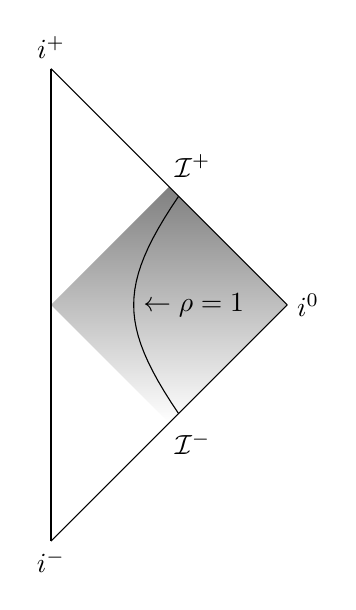
\begin{tikzpicture}[scale=1.5]
  \shade (0,0) -- (1,1) -- (2,0) -- (1,-1) -- (0,0);
  \draw (0,2) node[above] {$i^+$};
  \draw (0,-2) node[below] {$i^-$};
  \draw (2,0) node[right] {$i^0$};
  \draw (1.2,1) node[above] {$\mathcal{I}^+$};
  \draw (1.2,-1) node[below] {$\mathcal{I}^-$};
  \draw (0.7,0) node[right] {$\leftarrow \rho=1$};
  \draw (0,2) -- (0,-2);
  \draw (0,2) -- (2,0);
  \draw (0,-2) -- (2,0);
  \pgfmathsetmacro{\e}{1.5}   % eccentricity
  \pgfmathsetmacro{\a}{0.7}
  \pgfmathsetmacro{\b}{(\a*sqrt((\e)^2-1)}
  \draw plot[domain=-1:1] ({\a*cosh(\x)},{\b*sinh(\x)});
\end{tikzpicture} \caption{Minkowski spacetime may be divided up into radial ($\rho$) slices
isometric to 3D de Sitter spacetime as shown in the top panel. The
bottom panel shows the Penrose diagram of Minkowski spacetime. The
shaded region is the region bounded by $\rho=0$ and $\rho=\infty$.
In particular, $i^{\pm}$ are excluded from this region.}
\label{fig:coord}
\end{figure}

Before we begin our discussion of the representation theory of ${\rm SO(3,1)}$
in de Sitter and Minkowski spacetimes, we would like to present the
coordinate systems we employ and fix notation. A schematic plot of
the relevant hypersurfaces can be found in Fig.~\ref{fig:coord}.

We start with the 4d flat Minkowski spacetime labeled by coordinates
$(x^{0},x^{1},x^{2},x^{3})$ with the following metric
\[
\dd s^{2}=-(\dd x^{0})^{2}+(\dd x^{1})^{2}+(\dd x^{2})^{2}+(\dd x^{3})^{2}\,.
\]
We embed our 3D de Sitter spacetime as a hypersurface within the 4d
Minkowski spacetime. To do so we first switch to hyperbolic coordinates
$(t,\rho,\theta,\varphi)$ with $-\infty<t<\infty$, $\rho>0$, $0\le\theta<\pi$
and $0\le\varphi<2\pi$, defined by
\begin{align}
x^{0} & =\rho\sinh(t/\rho)\nonumber \\
x^{1} & =\rho\cos\theta\cosh(t/\rho)\nonumber \\
x^{2} & =\rho\sin\theta\cos\varphi\cosh(t/\rho)\nonumber \\
x^{3} & =\rho\sin\theta\sin\varphi\cosh(t/\rho)\,.\label{eq:embedding}
\end{align}
Note that these coordinates only cover the region of the Minkowski
spacetime defined by points $x^{\mu}$ where $x\cdot x>0$. The metric
then becomes
\[
\dd s^{2}=-\dd t^{2}+\frac{2t\,\dd\rho\,\dd t}{\rho}+\left(1-\frac{t^{2}}{\rho^{2}}\right)\dd\rho^{2}+\rho^{2}\cosh^{2}\left(\frac{t}{\rho}\right)\left(\dd\theta^{2}+\sin^{2}\theta\,\dd\varphi^{2}\right)\,.
\]
The d'Alembertian in this coordinate system looks rather complicated.
We therefore perform the following change of variables
\[
\eta=\frac{t}{\rho}
\]
and the metric takes the following simpler form
\[
\dd s^{2}=-\rho^{2}\dd\eta^{2}+\dd\rho^{2}+\rho^{2}\cosh^{2}\eta\left(\dd\theta^{2}+\sin^{2}\theta\,\dd\varphi^{2}\right)\,.
\]

A 3D de Sitter spacetime can then be embedded into this 4d Minkowski
spacetime as a hypersurface of constant $\rho=\ell$, where $\ell$
is the de Sitter length scale which we will set to unity in what follows.
On the 3D de Sitter spacetime the induced metric is simply
\[
\dd s^{2}=-\dd t^{2}+\cosh^{2}t\left(\dd\theta^{2}+\sin^{2}\theta\,\dd\varphi^{2}\right)\,.
\]
Through a stereographic projection we can parameterize the 2-sphere
covered by coordinates $(\theta,\varphi)$ with a complex variable
$z$, and obtain the Fubini-Study metric on the 2-sphere:
\[
\dd\theta^{2}+\sin^{2}\theta\,\dd\varphi^{2}=\frac{4\,\dd z\,\dd\bar{z}}{(1+|z|^{2})^{2}}\,.
\]
This allows us to rewrite the 3D de Sitter metric as
\begin{equation}
\dd s^{2}=-\dd t^{2}+\cosh^{2}t\,\frac{4\,\dd z\,\dd\bar{z}}{(1+|z|^{2})^{2}}\label{eq:3dds}
\end{equation}
and the 4d Minkowski metric in hyperbolic coordinates as
\[
\dd s^{2}=-\rho^{2}\dd\eta^{2}+\dd\rho^{2}+\rho^{2}\cosh^{2}\eta\,\frac{4\,\dd z\,\dd\bar{z}}{(1+|z|^{2})^{2}}\,.
\]


\section{3D de-Sitter Mode Functions}

\label{sec:dsmodes}

We start from the metric on the 3D de Sitter spacetime \eqref{eq:3dds}.
The isometry group of the 3D de Sitter spacetime is ${\rm SO(3,1)}$
which has 6 generators with real coefficients. The first step in building
a unitary representation of ${\rm SO(3,1)}$ on 3D de Sitter is to
solve the scalar field equation with mass $\mu$
\[
(\Delta-\mu^{2})\phi(t,z,\bar{z})=0
\]
where the d'Alembertian is defined in general as
\[
\Delta\phi=\frac{1}{\sqrt{|g|}}\partial_{i}(g^{ij}\sqrt{|g|}\partial_{j}\phi)\,.
\]
Here and in what follows we use Latin indices when we are referring
to the 3D de Sitter submanifold and use Greek indices when we are
dealing with the ambient 4d Minkowski spacetime. The d'Alembertian
is computed to be
\[
\Delta\phi=\left[-\partial_{t}^{2}-2(\tanh t)\partial_{t}+(\sech^{2}t)(1+|z|^{2})^{2}\partial_{z}\partial_{\bar{z}}\right]\phi\,.
\]
The massive scalar field equation therefore is
\[
\left(-\frac{\partial^{2}}{\partial t^{2}}-2\tanh t\frac{\partial}{\partial t}+\mathrm{sech}^{2}t\,(1+|z|^{2})^{2}\frac{\partial^{2}}{\partial z\partial\bar{z}}-\mu^{2}\right)\phi(t,z,\bar{z})=0\,.
\]
We can perform separation of variables as usual and write a mode function
as
\[
\phi_{lm}(t,z,\bar{z})=\phi_{l}(t)\,Y_{m}^{l}(z,\bar{z})
\]
where $m$ is a $j_{3}$ eigenvalue. The $Y_{m}^{l}$ are the standard
spherical harmonics \cite{kelvin1867treatise} in $(z,\bar{z})$
coordinates. They satisfy the eigenvalue equation
\[
(1+|z|^{2})^{2}\frac{\partial^{2}}{\partial z\partial\bar{z}}Y_{m}^{l}=-l(l+1)Y_{m}^{l}\,.
\]
Explicitly, we have
\[
Y_{m}^{l}(\theta,\varphi)=\sqrt{\frac{(2l+1)(l-m)!}{4\pi(l+m)!}}P_{l}^{m}(\cos\theta)e^{im\varphi}
\]
where
\[
P_{l}^{m}(x)=\frac{(1+x)^{m/2}}{(1-x)^{m/2}}\sum_{k=0}^{l}\frac{\left(\frac{1-x}{2}\right)^{k}(-l)_{k}(l+1)_{k}}{k!\,\Gamma(k-m+1)}\,.
\]
The coordinate transformation linking $(\theta,\varphi)$ and $(z,\bar{z})$
is
\[
(\sin\theta\,e^{i\varphi},\cos\theta)=\left(\frac{2z}{1+|z|^{2}},\frac{1-|z|^{2}}{1+|z|^{2}}\right)\,.
\]
It is easy to see that the spherical harmonics $Y_{l}^{m}(z,\bar{z})$
can be built out of homogeneous polynomials of the following three
variables
\[
F_{z}=\frac{2z}{1+|z|^{2}}\qquad F_{\bar{z}}=\frac{2\bar{z}}{1+|z|^{2}}\qquad F_{t}=\frac{1-|z|^{2}}{1+|z|^{2}}\,.
\]
We will later see that these three variables will appear in (\ref{eq:cartesian}).
One is then left to solve
\[
\left(\frac{\partial^{2}}{\partial t^{2}}+2\tanh t\frac{\partial}{\partial t}+l(l+1)\mathrm{sech}^{2}t+\mu^{2}\right)\phi_{l}(t)=0\,.
\]
This has the following two linearly independent solutions
\begin{equation}
\phi_{l,1}(t)=\mathrm{sech}t\,P_{l}^{\sqrt{1-\mu^{2}}}\left(\tanh t\right),\quad\phi_{l,2}(t)=\mathrm{sech}t\,Q_{l}^{\sqrt{1-\mu^{2}}}\left(\tanh t\right)\label{eq:basis}
\end{equation}
where $P$ and $Q$ are the associated Legendre functions of first
and second kind, respectively. We expect to get a unitary representation
corresponding to a general complex linear combination, one of which
will be the Euclidean vacuum (see Section \ref{sec:norm} and Appendix
\ref{app:euclidean}). Other combinations will generate modes around an
$\alpha$-vacuum \cite{PhysRevD.32.3136,GOLDSTEIN2003325,PhysRevD.69.023507}.

\section{Uplifting onto 4D Minkowski}

\label{sec:minkmodes}

To uplift the 3D de Sitter mode functions onto the 4d Minkowski spacetime
we consider the scalar field equation in 4d with mass $M$
\[
(\Box-M^{2})\Phi(\eta,\rho,z,\bar{z})=0\,.
\]
The d'Alembertian is computed to be
\[
\Box=-\frac{1}{\rho^{2}}(\partial_{\eta}^{2}+2\tanh\eta\,\partial_{\eta})+3\frac{\partial_{\rho}}{\rho}+\partial_{\rho}^{2}+\frac{\sech^{2}\eta\,(1+|z|^{2})^{2}\,\partial_{z}\partial_{\bar{z}}}{\rho^{2}}\,.
\]
Separating variables, the mode functions can be written as
\[
\Phi_{plm}(\eta,\rho,z,\bar{z})=\phi_{pl}(\eta)\,\psi_{p}(\rho)\,Y_{m}^{l}(z,\bar{z})
\]
where $l=0,1,\cdots$, $m=-l,\cdots,l$ and the range of the real
parameter $p$ will be discussed later. We find the differential equation
for $\phi_{pl}$ to be identical to the 3D de Sitter modes, except
that we replace $\mu$ with a real parameter $p$,
\[
\left(\partial_{\eta}^{2}+2(\tanh\eta)\partial_{\eta}+l(l+1)\sech^{2}\eta+p^{2}\right)\phi_{pl}(\eta)=0
\]
which has solutions \eqref{eq:basis} with the replacement $t\to\eta$
and $\mu\to p$.

The differential equation for $\psi_{p}$ therefore becomes
\[
\left(\partial_{\rho}^{2}+\frac{3}{\rho}\partial_{\rho}+\frac{p^{2}}{\rho^{2}}-M^{2}\right)\psi_{p}(\rho)=0\,.
\]
This has two independent solutions
\begin{equation}
\psi_{p,1}=\frac{I_{\sqrt{1-p^{2}}}(M\rho)}{\rho}\,,\qquad\psi_{p,2}=\frac{K_{\sqrt{1-p^{2}}}(M\rho)}{\rho}\label{eq:radialsol}
\end{equation}
where $I_{\alpha}$ and $K_{\alpha}$ are modified Bessel functions
of first and second kind, respectively.

\section{Klein-Gordon Norm and Orthonormality Conditions}

\label{sec:norm}

Before presenting the explicit form of our unitary principal series
representation we would like to first establish the orthonormalizability
of the 4d Minkowski mode functions. The mode functions are normalized
with respect to the Klein-Gordon norm, the most general form of which
is \cite{birrell1984quantum}
\begin{equation}
\langle f,g\rangle=-i\int_{\Sigma}\dd\Sigma\,n^{\lambda}(f\partial_{\lambda}g^{\star}-g^{\star}\partial_{\lambda}f)\,.\label{eq:kgnorm}
\end{equation}
Here $\Sigma$ is a spacelike surface, $n^{\lambda}$ is a timelike
unit vector field normal to $\Sigma$ and $d\Sigma$ is the volume
element in $\Sigma$. This norm is time-independent, and in principle
can be evaluated on any Cauchy slice. Here, for convenience we choose
the $\eta=\eta_{0}$ slice, where $\eta_{0}$ is an arbitrary constant.
On the 4d Minkowski spacetime with coordinate system $(\eta,\rho,\theta,\varphi)$
this then becomes
\[
\langle f,g\rangle=-i\int_{\rho}\int_{S^{2}}(f\partial_{\eta}g^{\star}-g^{\star}\partial_{\eta}f)|_{\eta=\eta_{0}}\,(\cosh^{2}\eta_{0})\,\rho\,\dd\rho\,\dd\Omega
\]
where $\dd\Omega$ is the area element of the unit 2-sphere $S^{2}$.
Given that our mode functions are separable $\Phi_{plm}(\eta,\rho,z,\bar{z})=\phi_{pl}(\eta)\psi_{p}(\rho)Y_{m}^{l}(z,\bar{z})$
we can further evaluate this norm to obtain
\begin{align*}
\langle\Phi_{plm},\Phi_{p'l'm'}\rangle= & -i\,\left(\phi_{pl}(\eta_{0})\dot{\phi}_{p'l'}^{\star}(\eta_{0})-\phi_{p'l'}^{\star}(\eta_{0})\dot{\phi}{}_{pl}(\eta_{0})\right)\,\left(\cosh^{2}\eta_{0}\right)\\
 & \qquad\times\int_{0}^{\infty}\psi_{p}(\rho)\psi_{p'}^{\star}(\rho)\,\rho\,\dd\rho\int_{S^{2}}Y_{m}^{l}(z,\bar{z})Y_{m'}^{\star l'}(z,\bar{z})\,\dd\Omega
\end{align*}
where $\dot{\phi}(\eta)=\partial_{\eta}\phi$. The orthonormality
of the spherical harmonics allows us to conclude that
\[
\int_{S^{2}}Y_{m}^{l}(z,\bar{z})Y_{m'}^{\star l'}(z,\bar{z})\,\dd\Omega=\delta_{ll'}\delta_{mm'}\,.
\]
For the $\rho$ integral, note that multiplying the differential equation
satisfied by $\psi_{p}$ with $\psi_{p'}^{\star}$ gives
\[
\psi''_{p}\psi_{p'}^{\star}+\frac{3}{\rho}\psi'_{p}\psi_{p'}^{\star}+\left(\frac{p^{2}}{\rho^{2}}-M^{2}\right)\psi_{p}\psi_{p'}^{\star}=0
\]
where $\psi'=\partial_{\rho}\psi$. Likewise swapping $\psi_{p}\leftrightarrow\psi_{p'}^{*}$
and subtracting we have
\[
-\frac{p^{2}-p'^{2}}{\rho^{2}}\psi_{p}\psi_{p'}^{\star}=\psi''_{p}\psi_{p'}^{\star}-\psi_{p'}^{\star''}\psi_{p}+\frac{3}{\rho}\psi'_{p}\psi_{p'}^{\star}-\frac{3}{\rho}\psi_{p'}^{\star'}\psi_{p}\,.
\]
Integrating, we have
\[
-(p^{2}-p'^{2})\int_{0}^{\infty}\psi_{p}\psi_{p'}^{\star}\,\rho\,\dd\rho=\int_{0}^{\infty}\dd\rho\,[\rho^{3}(\psi''_{p}\psi_{p'}^{\star}-\psi_{p'}^{\star''}\psi_{p})+3\rho^{2}(\psi'_{p}\psi_{p'}^{\star}-\psi_{p'}^{\star'}\psi_{p})]\,.
\]
The integral on the right hand side can be integrated by parts to
yield
\begin{equation}
-(p^{2}-p'^{2})\int_{0}^{\infty}\psi_{p}\psi_{p'}^{\star}\,\rho\,\dd\rho=[\rho^{3}(\psi'_{p}\psi_{p'}^{\star}-\psi_{p'}^{\star'}\psi_{p})]\Big|_{0}^{\infty}\,.\label{eq:norm-int}
\end{equation}

The modified Bessel functions have the following mirror symmetry
\[
I_{\alpha}^{\star}(z)=I_{\alpha^{\star}}(z^{\star})\qquad K_{\alpha}^{\star}(z)=K_{\alpha^{\star}}(z^{\star})\,.
\]
At $z=+\infty$, $I_{\alpha}(z)\sim e^{z}$ which increases exponentially
while $K_{\alpha}(z)\sim e^{-z}$ which decreases exponentially. We
therefore discard the $\psi_{p,1}$ set of solutions as these modes
are not normalizable and study the \eqref{eq:radialsol} solutions
$\psi_{p,2}$. We begin by considering the case $p^{2}>1$ and take
the branch $\sqrt{1-p^{2}}=i\sqrt{p^{2}-1}$. Let us define $\alpha=\sqrt{p^{2}-1}$
and henceforth we will drop the 2 subscript on $\psi_{p,2}$. Near
$z=0$, the expansion
\[
K_{\nu}(z)=2^{\nu-1}\Gamma(\nu)z^{-\nu}+2^{-\nu-1}\Gamma(-\nu)z^{\nu}+\cdots
\]
allows us to evaluate the surface term to give
\begin{align}
 & \lim_{\rho\to0}\rho^{3}\left(\psi'_{p}\psi_{p'}^{*}-\psi_{p'}^{*'}\psi_{p}\right)=\nonumber \\
 & \quad\lim_{\rho\to0}i(\alpha+\alpha')2^{-2}\left(\Gamma(i\alpha')\Gamma(-i\alpha)(M\rho/2)^{i(\alpha-\alpha')}-\Gamma(i\alpha)\Gamma(-i\alpha')(M\rho/2)^{-i(\alpha-\alpha')}\right)\label{eq:surfaceterm}
\end{align}
treating the rapidly oscillating terms in $\alpha$ as vanishing in
the sense of a distribution. For $\rho\to0$, this is proportional
to a sinc representation of the Dirac delta function
\[
\lim_{\rho\to0}\rho^{3}\left(\psi'_{p}\psi_{p'}^{*}-\psi_{p'}^{*'}\psi_{p}\right)=-\frac{\alpha\Gamma(i\alpha)\Gamma(-i\alpha)}{2}\sin\left[(\alpha-\alpha')\log(M\rho/2)\right]
\]
which gives
\[
\int_{0}^{\infty}\psi_{p}\psi_{p'}^{\star}\,\rho\,\dd\rho=\frac{\Gamma(i\alpha)\Gamma(-i\alpha)}{4}\lim_{C\to\infty}\frac{\sin[C(\alpha-\alpha')]}{\alpha-\alpha'}
\]
where we have set $C=\log(M\rho/2)$. Using the following identity
\[
\lim_{C\to\infty}\frac{\sin(Cx)}{x}=\pi\delta(x)
\]
we then have
\begin{equation}
\int_{0}^{\infty}\psi_{p}\psi_{p'}^{\star}\,\rho\,\dd\rho=\frac{\pi\Gamma(i\alpha)\Gamma(-i\alpha)}{4}\delta(\alpha-\alpha')=\frac{\pi^{2}}{4p\sinh\left(\pi\sqrt{p^{2}-1}\right)}\delta\left(p-p'\right)\,.\label{eq:radialnorm}
\end{equation}
 For $0\le p^{2}<1$, instead of oscillating terms in eq.~\ref{eq:surfaceterm}
we have power-law divergencies, and the mode functions $\psi_{p}$
in this case again are not normalizable.

To conclude, the normalizable radial mode functions arise from $\psi_{p,2}$
in \eqref{eq:radialsol} with $p^{2}>1$. The $p$-dependent prefactor
in \eqref{eq:radialnorm} may then be absorbed into the normalization
of these functions. We assume this has been done, and in the interest
of notational clarity we will from now use $\psi_{p}$ to denote the
normalized radial mode functions. The normalized radial mode functions
in this case will satisfy the following
\begin{equation}
\int_{0}^{\infty}\psi_{p}\psi_{p'}^{\star}\,\rho\,\dd\rho=\delta(p-p')\,.\label{eq:radialinnerprod}
\end{equation}

For the $\eta$ dependence, we form the following linear combination
of $\phi_{pl,1}$ and $\phi_{pl,2}$ to obtain
\[
\phi_{pl}=\frac{i\pi}{2}\phi_{pl,1}+\phi_{pl,2}
\]
which, as we will show in Appendix \ref{app:euclidean}, are the (unnormalized)
modes corresponding to the 4d Minkowski vacuum. Using
\[
\frac{\partial P_{\nu}^{\mu}}{\partial z}=\frac{\nu zP_{\nu}^{\mu}(z)-(\mu+\nu)P_{\nu-1}^{\mu}(z)}{z^{2}-1}\qquad\frac{\partial Q_{\nu}^{\mu}}{\partial z}=\frac{\nu zQ_{\nu}^{\mu}(z)-(\mu+\nu)Q_{\nu-1}^{\mu}(z)}{z^{2}-1}
\]
and
\[
P_{\nu}^{\mu}(0)=\frac{\pi^{1/2}2^{\mu}}{\Gamma\left(\frac{1-\mu-\nu}{2}\right)\Gamma\left(\frac{\nu-\mu}{2}+1\right)}\qquad Q_{\nu}^{\mu}(0)=-\frac{\pi^{3/2}2^{\mu-1}\tan\frac{\pi(\mu+\nu)}{2}}{\Gamma\left(\frac{1-\mu-\nu}{2}\right)\Gamma\left(\frac{\nu-\mu}{2}+1\right)}
\]
we can evaluate the $\eta$-dependent part of the Klein-Gordon norm
to obtain
\[
-i[\phi_{pl}(\eta_{0})\phi_{pl}^{\star'}(\eta_{0})-\phi_{pl}^{\star}(\eta_{0})\phi'_{pl}(\eta_{0})](\cosh^{2}\eta_{0})=\pi e^{-\pi\sqrt{p^{2}-1}}
\]
which does not depend on $\eta_{0}$ due to conservation of the Klein-Gordon
norm. We can therefore normalize the modes $\phi_{pl}$ by replacing
\[
\phi_{pl}\to\frac{e^{\frac{\pi}{2}\sqrt{p^{2}-1}}}{\pi^{1/2}}\phi_{pl}\,.
\]
In what follows we will assume that this has been done and in the
interest of notational simplicity we will use $\phi_{pl}$ to denote
the normalized modes.

To summarize, for $p^{2}>1$ we have constructed mode functions of
the 4d Klein-Gordon equation corresponding to the Minkowski vacuum,
which when restricted to the de Sitter slice $\rho=1$ correspond
to the Euclidean vacuum of the 3D de Sitter spacetime. These modes
$\Phi_{plm}(\eta,\rho,z,\bar{z})=\phi_{pl}(\eta)\psi_{p}(\rho)Y_{m}^{l}(z,\bar{z})$
are normalized with respect to to the Klein-Gordon norm (\ref{eq:kgnorm})
with the following orthonormality condition
\[
\langle\Phi_{plm},\Phi_{p'l'm'}\rangle=\delta(p-p')\delta_{ll'}\delta_{mm'}\,.
\]
For $0\le p^{2}<1$, the radial mode functions are not normalizable.

\section{Unitary Principal Series Representation}

\label{sec:ups} We are now in a position to build the unitary principal
series representation of ${\rm SO(3,1)}$ which acts on the ${\rm dS_{3}}$/${\rm M_{4}}$
mode functions. Since the action of ${\rm SO(3,1)}$ on ${\rm M_{4}}$
leaves the radial coordinate $\rho$ invariant, the actions is identical
on both ${\rm dS_{3}}$ mode functions and on ${\rm M_{4}}$ mode
functions. For simplicity of presentation we will focus on ${\rm dS_{3}}$
modes, but all equations in this section carry over to the ${\rm M_{4}}$
modes trivially.

On the past and future null infinities $\mathcal{I^{\pm}}$ of the
3D de Sitter spacetime, the Killing vectors can be written as conformal
Killing vectors of the spatial 2-sphere
\[
L_{n}=-z^{n+1}\frac{\partial}{\partial z},\,\bar{L}_{n}=-\bar{z}^{n+1}\frac{\partial}{\partial\bar{z}}
\]
where $n=0,\pm1$. However one should use caution in applying this
formula. It is correct when acting on the metric, or massless scalars,
but as we will see there will be additional terms that must be added
depending on the class of functions or fields considered. General
complex combinations of these vectors will not preserve the desired
reality conditions, so we will need to be careful to construct the
correct 6 independent generators that will appear with real coefficients.

To extend these into the bulk of de Sitter it is helpful to arrange
them into an ${\rm SO(3)}$ corresponding to the isometries of the
spatial slices. With the convention $g=\exp(i\theta J)$ we find the
generators:
\begin{align*}
J_{1} & =\frac{i}{2}\left(L_{-1}+L_{1}+\bar{L}_{-1}+\bar{L}_{1}\right)\\
J_{2} & =\frac{1}{2}\left(L_{-1}-L_{1}-\bar{L}_{-1}+\bar{L}_{1}\right)\\
J_{3} & =L_{0}-\bar{L}_{0}\,.
\end{align*}
These immediately extend into the bulk without time dependent contributions.
This also allows us to read off the conjugation condition to be imposed
on the generators. Since the $J_{k}$ are Hermitian we require
\[
L_{n}^{\dagger}=-\bar{L}_{n},\qquad\bar{L}_{n}^{\dagger}=-L_{n}\,.
\]

The time-dependent Killing vectors take the form
\[
K=F\frac{\partial}{\partial t}+\frac{1}{2}\left(1+z\bar{z}\right)^{2}\tanh t\,\left(\partial_{\bar{z}}F\right)\frac{\partial}{\partial z}+\frac{1}{2}\left(1+z\bar{z}\right)^{2}\tanh t\,\left(\partial_{z}F\right)\frac{\partial}{\partial\bar{z}}
\]
where $F$ is one of the three solutions
\begin{equation}
F_{z}=\frac{2z}{1+|z|^{2}}\qquad F_{\bar{z}}=\frac{2\bar{z}}{1+|z|^{2}}\qquad F_{t}=\frac{1-|z|^{2}}{1+|z|^{2}}\,.\label{eq:cartesian}
\end{equation}
At $\mathcal{I}^{+}$ these reduce to
\begin{align*}
\tilde{K}_{1} & =L_{1}-\bar{L}_{-1}\\
\tilde{K}_{2} & =\bar{L}_{1}-L_{-1}\\
\tilde{K}_{3} & =L_{0}+\bar{L}_{0}
\end{align*}
when acting on the metric. It is convenient to assemble these into
Hermitian linear combinations:
\begin{align*}
K_{1} & =\frac{1}{2}\left(L_{1}-\bar{L}_{-1}-\bar{L}_{1}+L_{-1}\right)\\
K_{2} & =\frac{i}{2}\left(\bar{L}_{1}-L_{-1}+L_{1}-\bar{L}_{-1}\right)\\
K_{3} & =-i\left(L_{0}+\bar{L}_{0}\right)
\end{align*}
which at a general spacetime point become
\begin{align}
K_{1} & =\frac{1}{2}\left(\frac{2(z-\bar{z})}{1+|z|^{2}}\frac{\partial}{\partial t}-\tanh t\left(\left(z^{2}+1\right)\frac{\partial}{\partial z}-\left(\bar{z}^{2}+1\right)\frac{\partial}{\partial\bar{z}}\right)\right)\nonumber \\
K_{2} & =\frac{i}{2}\left(\frac{2(z+\bar{z})}{1+|z|^{2}}\frac{\partial}{\partial t}-\tanh t\left(\left(z^{2}-1\right)\frac{\partial}{\partial z}+\left(\bar{z}^{2}-1\right)\frac{\partial}{\partial\bar{z}}\right)\right)\nonumber \\
K_{3} & =-i\left(\frac{1-|z|^{2}}{1+|z|^{2}}\frac{\partial}{\partial t}-\tanh t\left(z\frac{\partial}{\partial z}+\bar{z}\frac{\partial}{\partial\bar{z}}\right)\right)\,.\label{eq:bulkgen}
\end{align}
Note the generators satisfy the canonical Lorentz algebra
\begin{align*}
[J_{i},J_{j}] & =i\epsilon_{ijk}J_{k}\\{}
[J_{i},K_{j}] & =i\epsilon_{ijk}K_{k}\\{}
[K_{i},K_{j}] & =-i\epsilon_{ijk}J_{k}\,.
\end{align*}

On the three-dimensional de Sitter mode functions (\ref{eq:basis})
the generators (\ref{eq:bulkgen}) take the simplified form
\begin{align}
K_{1} & =\frac{1}{2}\left(\frac{2(z-\bar{z})}{1+|z|^{2}}\left(2h_{+}-2\right)-\left(\left(z^{2}+1\right)\frac{\partial}{\partial z}-\left(\bar{z}^{2}+1\right)\frac{\partial}{\partial\bar{z}}\right)\right)\nonumber \\
K_{2} & =\frac{i}{2}\left(\frac{2(z+\bar{z})}{1+|z|^{2}}\left(2h_{+}-2\right)-\left(\left(z^{2}-1\right)\frac{\partial}{\partial z}+\left(\bar{z}^{2}-1\right)\frac{\partial}{\partial\bar{z}}\right)\right)\nonumber \\
K_{3} & =-i\left(\frac{1-|z|^{2}}{1+|z|^{2}}\left(2h_{+}-2\right)-\left(z\frac{\partial}{\partial z}+\bar{z}\frac{\partial}{\partial\bar{z}}\right)\right)\label{eq:bulkgenprin}
\end{align}
where we define
\[
2h_{\pm}=\frac{d-1}{2}\pm\sqrt{\left(\frac{d-1}{2}\right)^{2}-\mu^{2}}=1\pm\sqrt{1-\mu^{2}}\,.
\]
To check this we note that the group of rotations ${\rm SO(3)}$ acts
straightforwardly in the basis \eqref{eq:basis}. The rotation generators
also rotate the $K_{i}$ amongst themselves, so we can focus on the
action of say $K_{3}$ on the mode functions \eqref{eq:basis}. It
is then straightforward to check that
\[
\frac{\partial}{\partial t}\phi_{l=0}=2(h_{+}-1)\phi_{l=1}
\]
which holds for the solutions $\phi_{l,1}$ and $\phi_{l,2}$ of \eqref{eq:basis}
independently and determines the prefactors that appear in \eqref{eq:bulkgenprin}.
Likewise, when acting on the four-dimensional Minkowski modes the
generators take the exact same expression with $\mu$ replaced by
$p$.

To confirm the generators match the principal series we will use the
representation of ${\rm SO(3,1)}$ on functions $L^{2}(S^{2})$. Note
this differs from the more common representation on functions $L^{2}(\mathbb{C})$,
which would be applicable to the flat slicing of de Sitter. Likewise
there is a representation on $L^{2}(H^{2})$, though we won't need
that here. The upshot of these different realizations of the principal
series is that the extra terms in \eqref{eq:bulkgenprin} take completely
different forms.

To realize the representation we consider the cone $C_{+}^{3}$ embedded
in 4d Minkowski spacetime, where
\[
x_{1}^{2}+x_{2}^{2}+x_{3}^{2}-x_{0}^{2}=0\,.
\]
We then consider the slice through the cone where $x_{0}=1$. This
slice is an $S^{2}$ which may be parameterized by coordinates $z$
above using the Fubini-Study metric. The cone maps into itself under
${\rm SO(3,1)}$. The principal series may be defined as functions
on the slice that behave as \cite{vilenkin1992representation}
\begin{equation}
(T^{\sigma}(g)f)(z)=\alpha(z,g)^{\sigma}f\left(\frac{g^{-1}\cdot z}{\alpha(z,g)}\right)\label{eq:prindef}
\end{equation}
where $g$ is a ${\rm SO(3,1)}$ group element, and $\alpha(z,g)$
is defined to be the rescaling factor needed to return $g^{-1}\cdot x^{\mu}$
to the slice $x_{0}=1$. The action of ${\rm SO(3,1)}$ on $z$ is
the usual fraction linear transformation, but the factor $\alpha$
depends on which realization of the principal series we are considering.
To write the action of ${\rm SL}(2,\mathbb{C})$ on the Minkowski
coordinates it is helpful to use the familiar representation
\[
x^{\mu}=\frac{1}{2}\mathrm{Tr}\left(M\sigma^{\mu}\right),\qquad M=\left(\begin{array}{cc}
x^{0}+x^{3} & x^{1}-ix^{2}\\
x^{1}+ix^{2} & x^{0}-x^{3}
\end{array}\right),\qquad\sigma^{\mu}=\left(\mathbbm{1},\sigma^{i}\right)
\]
where $\sigma^{i}$ are the Pauli matrices. Then an ${\rm SL}(2,\mathbb{C})$
transformation acts as
\[
M'=SMS^{\dagger}\,.
\]
To rescale back to the slice $x^{0}=1$ we rescale to
\[
\tilde{M}'=\frac{M'}{\frac{1}{2}\mathrm{Tr}\left(M'\right)}\,.
\]
Finally, the coordinates on the 2-sphere $x^{0}=1$ are matched with
the Fubini-Study coordinates via
\begin{align*}
x^{1}+ix^{2} & =\frac{2z}{1+|z|^{2}}\\
x^{1}-ix^{2} & =\frac{2\bar{z}}{1+|z|^{2}}\\
x^{3} & =\frac{1-|z|^{2}}{1+|z|^{2}}\,.
\end{align*}
From these equations we can read off the factor $\alpha$ and determine
the action of the $z$ coordinate. For
\[
S=\left(\begin{array}{cc}
a & b\\
c & d
\end{array}\right)\,,
\]
the fractional linear transformation is
\[
z'=\frac{dz+c}{bz+a}\,.
\]

Since we know the group of rotations acts in a straightforward way
on the spherical harmonics, it suffice to consider one of the boost
generators to check the matching of the generators. To do this we
Taylor expand \eqref{eq:prindef} for a group element of the form
$g=\exp(ik_{3}\epsilon)$. Plugging in the above relations gives
\[
K_{3}=-i\left(\frac{1-|z|^{2}}{1+|z|^{2}}\sigma-\left(z\frac{\partial}{\partial z}+\bar{z}\frac{\partial}{\partial\bar{z}}\right)\right)\,.
\]
We therefore identify the scalar field representation with a principal
series representation where $\sigma=-2h_{-}$. We have $\sigma=-1+i\sqrt{\mu^{2}-1}$
in the notation of \cite{vilenkin1992representation}. We note the
equivalence of the representations under the replacement $h_{+}\to h_{-}$
and $2h_{+}-2=-2h_{-}$. For the principal series, the inner product
is simply the usual integral over the 2-sphere in Fubini-Study coordinates
which matches the Klein-Gordon norm up to a constant factor. For $0<\mu^{2}<1$
we have the complementary series representations and the above results
extend straightforwardly to that case.

\section{Relation to Previous Work}

\label{sec:psrep}

Here we show the mode functions computed in Ref.~\cite{Pasterski:2017kqt}
form a non-unitary highest-weight representation, and therefore do
not produce a unitary principal series representation of $SO(3,1)$.
To do so we first show that the generators of the special conformal
transformations annihilate a mode function corresponding to the highest
weight of the representation. The mode functions (eq.~2.19 of \cite{Pasterski:2017kqt})
are parameterized by the tuple $(\Delta,\vec{w})$ where $\Delta$
is in general a complex number and $\vec{w}=(w_{x},w_{y})\in\mathbb{R}^{2}$.
These mode functions are
\begin{equation}
\phi_{\Delta}^{\pm}(X^{\mu};\vec{w})=\frac{4\pi}{(im)}\frac{(\sqrt{-X^{2}})^{\Delta-1}}{(-q(\vec{w})\cdot X\mp i\epsilon)^{\Delta}}K_{\Delta-1}(m\sqrt{X^{2}})\,.\label{eq:psmode}
\end{equation}
Here $X^{\mu}$ are the usual flat coordinates of the 4d Minkowski
spacetime ${\rm M_{4}}$. The $q^{\mu}(\vec{w})$ is the following
4-vector
\[
q^{\mu}(\vec{w})=(1+|\vec{w}|^{2},2\vec{w},1-|\vec{w}|^{2})\,.
\]
The conformal group ${\rm SO(3,1)}$ acts on the space of scalar functions
defined on ${\rm M_{4}\times\mathbb{R}^{2}}$ by acting on ${\rm M_{4}}$
with the usual Lorentz transformation and on $\mathbb{R}^{2}$ with
the 2D conformal transformations (2D translations, 2D rotations, dilatations
and special conformal transformations):
\[
\phi_{\Delta}(X^{\mu};\vec{w})\to\phi_{\Delta}(\Lambda^{\mu}{}_{\nu}X^{\nu};\vec{w}'(\vec{w}))\,.
\]
Here $\Lambda^{\mu}{}_{\nu}$ is the Lorentz transformation corresponding
to the ${\rm SO(3,1)}$ group element, and the $\vec{w}'(\vec{w})$
is the conformal transformation corresponding to the ${\rm SO(3,1)}$
element. For special conformal transformation, it is
\[
\vec{w}'=\frac{\vec{w}+|\vec{w}|^{2}\vec{b}}{1+2\vec{b}\cdot\vec{w}+|\vec{b}|^{2}|\vec{w}|^{2}}\,.
\]
These are labeled by a vector $\vec{b}\in\mathbb{R}^{2}$.

Consider an infinitesimal group element near the identity
\[
\Lambda^{\mu}{}_{\nu}=\delta_{\nu}^{\mu}+(\delta\Lambda)^{\mu}{}_{\nu}
\]
this has the corresponding infinitesimal transformation on $\mathbb{R}^{2}$
\[
\vec{w}'=\vec{w}+\delta\vec{w}\,.
\]
In particular, for the special conformal transformation parameterized
by an infinitesimal $\vec{b}$ we have the infinitesimal transformation
\[
\vec{w}'=\vec{w}-2(\vec{w}\cdot\vec{b})\vec{w}+|\vec{w}|^{2}\vec{b}\,.
\]
Following the conventions of \cite{Pasterski:2017kqt} this corresponds
to the infinitesimal Lorentz transformation where
\[
(\delta\omega)^{0}{}_{i}=(\delta\omega)^{i}{}_{0}=(\delta\omega)^{3}{}_{i}=-(\delta\omega)^{i}{}_{3}=b_{i}
\]
with all other components being zero. Here $i=x,y$ labels the indices
of $\mathbb{R}^{2}$. In other words we have
\[
\begin{bmatrix}X'^{0}\\
X'^{i}\\
X'^{3}
\end{bmatrix}=\begin{bmatrix}X^{0}\\
X^{i}\\
X^{3}
\end{bmatrix}+\begin{bmatrix}b_{i}X^{i}\\
b^{i}(X^{0}-X^{3})\\
b_{i}X^{i}
\end{bmatrix}\,.
\]
Taylor-expanding $\phi_{\Delta}(\Lambda^{\mu}{}_{\nu}X^{\nu};\vec{w}'(\vec{w}))$
and substituting the expressions for $\delta\omega$ and $\delta\vec{w}$
above, we have
\begin{align*}
\phi_{\Delta}(\Lambda^{\mu}{}_{\nu}X^{\nu};\vec{w}'(\vec{w})) & =\phi_{\Delta}(X^{\mu}+\left(\delta\omega\right)_{\enskip\nu}^{\mu}X^{\nu};\vec{w}+\delta\vec{w})\\
 & =\phi_{\Delta}(X^{\nu};\vec{w})+\left(\delta\omega\right)_{\enskip\nu}^{\mu}X^{\nu}\left(\frac{\partial}{\partial X^{\mu}}\phi_{\Delta}\right)+\delta\vec{w}\cdot\left(\frac{\partial}{\partial\vec{w}}\phi_{\Delta}\right)\\
 & =\phi_{\Delta}(X^{\nu};\vec{w})+b_{i}X^{i}\left(\frac{\partial}{\partial X^{0}}+\frac{\partial}{\partial X^{3}}\right)\phi_{\Delta}+b^{i}(X^{0}-X^{3})\left(\frac{\partial}{\partial X^{i}}\phi_{\Delta}\right)\\
 & \qquad+\left(-2(\vec{w}\cdot\vec{b})\vec{w}+|\vec{w}|^{2}\vec{b}\right)\cdot\left(\frac{\partial}{\partial\vec{w}}\phi_{\Delta}\right)\,.
\end{align*}
For infinitesimal $\vec{b}$ this evaluates to
\begin{equation}
\delta\phi_{\Delta}=\frac{8\pi\Delta}{im}\vec{b}\cdot\vec{w}\frac{\left(\sqrt{-X^{2}}\right){}^{\Delta-1}}{(-q(\vec{w})\cdot X\mp i\epsilon)^{\Delta}}K_{\Delta-1}\left(m\sqrt{X^{2}}\right)\,.\label{eq:lxpsmode}
\end{equation}
In particular, the special conformal transformations annihilate the
mode functions when the weight $\vec{w}=(0,0)$. This implies \cite{doi:10.1142/9789813149441_0001}
that the mode functions (\ref{eq:psmode}) form a highest-weight representation
of $SO(3,1)$, and since $SO(3,1)$ has only non-unitary highest-weight
representations, these mode functions cannot form a unitary principal
series.

\section{Discussion}

\label{sec:further} The results of the previous sections lead to
a proposal for a holographic mapping between the 3D de Sitter modes
and conformal operators on a two-sphere. Likewise, the construction
may be lifted to 4D Minkowski spacetime.

\begin{comment}
In the context of celestial sphere amplitudes \cite{deBoer:2003vf,Kapec:2014opa,Kapec:2016jld,Cheung:2016iub}
it is tempting to use our 4D Minkowski spacetime mode functions as
a conformal basis of wavefunctions against which all conformally invariant
amplitudes can be decomposed.
\end{comment}


\subsection{Holographic Mapping Between 3D de-Sitter and a Euclidean 2-Sphere}

For the case of a flat slicing, it was possible to define a bulk-to-boundary
map and its inverse map \cite{Chatterjee:2015pha} via a construction
reminiscent of the LSZ reduction formula in asymptotically flat spacetime
\cite{Lehmann:1954rq}. That construction does not extend immediately
to the case of the sphere slicing, but we will see the Klein-Gordon
inner product defined above can still be used to extract a natural
set of operators living on the 2-sphere.

We work with a scalar bulk field of mass $\mu$
\begin{equation}
\phi(t,z,\bar{z})=\sum_{l=0}^{\infty}\sum_{m=-l}^{l}a_{lm}\phi_{lm}(t,z,\bar{z})+a_{lm}^{\dagger}\phi_{lm}^{\dagger}(t,z,\bar{z})\label{eq:modeexpan}
\end{equation}
where $\phi_{lm}$ is defined using the Euclidean vacuum modes \eqref{eq:evacmode}
and $a_{lm}$ and $a_{lm}^{\dagger}$ are standard creation/annihilation
operators. Let us consider a late-time sphere at $t=T$ and build
the following inner product using the Klein-Gordon inner product in
3D de Sitter spacetime
\[
\mathcal{O}_{lm}=\left\langle \phi_{lm}(t),\phi(t,z,\bar{z})\right\rangle _{t=T}
\]
which identifies $\mathcal{O}_{lm}=a_{lm}$. Likewise one can define
$\mathcal{O}_{lm}^{\dagger}=a_{lm}^{\dagger}$. One may view this
mapping as a holographic map, with $l,m$ being dual variables to
the coordinates on the 2-sphere $z,\bar{z}$. The formula \eqref{eq:modeexpan}
can then be viewed as the inverse mapping reconstructing the bulk
field in terms of boundary operators. The boundary operators will
obey their usual commutation relations, and at the same time will
transform as a representation of the unitary principal series as described
above. All the above is established at the level of free field theory.
Once interactions are included it seems difficult to view the resulting
boundary theory as any kind of conventional field theory \cite{PhysRevD.96.066031}.

\subsection{Holographic Mapping Between Celestial Sphere and 4D Minkowski}

This procedure can be extended to the 4D Minkowski case. However we
will now have a continuous spectrum of allowed conformal weights $\Delta$
corresponding to the continuous spectrum of radial quantum numbers
$p$. For a scalar field we can use the orthogonality of the radial
mode functions \eqref{eq:radialinnerprod} to project onto a particular
$p$ eigenvalue and then follow the procedure of the previous subsection
to build a boundary operator. The mode expansion of the bulk field
is now
\[
\Phi(\eta,\rho,z,\bar{z})=\sum_{l=0}^{\infty}\sum_{m=-l}^{l}\int_{1}^{\infty}dp\left(a_{plm}\Phi_{plm}(\eta,\rho,z,\bar{z})+a_{plm}^{\dagger}\Phi_{plm}^{\dagger}(\eta,\rho,z,\bar{z})\right)
\]
where $a_{plm}$ and $a_{plm}^{\dagger}$ are annihilation and creation
operators. Again we can define an operator on the celestial 2-sphere
by constructing
\[
\mathcal{O}_{\Delta_{p},lm}=\left\langle \Phi_{plm}(\eta,\rho,z,\bar{z}),\Phi(\eta,\rho,z,\bar{z})\right\rangle =a_{plm}
\]
where the operator transforms as a unitary principal series representation
parameterized by $\Delta_{p}$. Likewise one may define a conjugate
operator $\mathcal{O}_{\Delta_{p},lm}^{\dagger}=a_{plm}^{\dagger}$.
We can therefore interpret this as a holographic map between the bulk
4D Minkowski spacetime and the boundary 2D celestial sphere. One ends
up with a continuous family of boundary operators labelled by the
radial quantum number $p$. As above, it is not clear how the construction
extends to interacting theories.

\chapter{Conformal Wavefunctions for Graviton Amplitudes}\label{chap:gravitons}
Building on the results of the previous chapter, it is of interest to study the
representations of the $\rm SO(3,1)$ group associated with gravitons. To reduce the equation of
motion to a Schr\"odinger-like equation it is necessary to impose a
non-covariant gauge condition. Using these solutions, leading-order
gauge invariant Weyl scalars are then computed and decomposed into
families of unitary principal series representations. An invertible
holographic mapping is constructed between these unitary principal
series operators and massless spin-2 perturbations of flat spacetime.

\section{Introduction}

In the previous chapter, massive scalar fields in 4D
Minkowski spacetime were decomposed into modes on 3D de-Sitter spacetime
slices where they form unitary principal series representations of
${\rm SO(3,1)}$. This study was motivated by the program of \cite{Pasterski:2016qvg}
where the goal is to formulate gravity in asymptotically flat spacetime
as a theory on the celestial sphere with conformal symmetry. In this
chapter we extend this construction to massless spin-2 particles, or
gravitons, in 4D Minkowski spacetime. To this end, we consider linearized
gravitational waves living in flat 4D background spacetime with the
standard spherical coordinates. The background metric is simply
\[
g_{\mu\nu}=\diag(-1,1,r^{2},r^{2}\sin^{2}\theta)
\]
Following the notations in \cite{Bernar:2014lna}, from now on indices
$a,b,c,\ldots$ refer to the ``orbit'' spacetime labeled by the
coordinates $(t,r)$, and $i,j,k,\ldots$ refer to the 2-sphere labeled
by $(\theta,\varphi)$. In other words, we write the background metric
as
\[
g_{\mu\nu}\,\dd x^{\mu}\dd x^{\nu}=g_{ab}\,\dd y^{a}\dd y^{b}+r^{2}\,\dd\sigma^{2}
\]
where $g_{ab}=\diag(-1,1)$ and $\dd\sigma^{2}=\gamma_{ij}\,\dd z^{i}\dd z^{j}=\dd\theta^{2}+\sin^{2}\theta\,\dd\varphi^{2}$.

For Minkowski spacetime in four dimensions, the gravitational perturbations
can be expanded in terms of both the scalar and the vector spherical
harmonics defined on the 2-sphere. These are also known as the ``even''
and ``odd'' waves in \cite{PhysRev.108.1063}, and will automatically
have the desired transformation properties under the rotation group
${\rm SO(3)}$. However, as we shall see, the specific gauge conditions
that we will choose in what follows are not Lorentz covariant, and
therefore these metric perturbations do not transform as tensors under
the full ${\rm SO(3,1)}$ group. To remedy this, we consider the Newman-Penrose
formalism \cite{doi:10.1063/1.1724257} of general relativity and
construct leading-order gauge-invariant scalars known as the Weyl
scalars. These scalars can then be mapped onto the celestial sphere
through a generalization of the method described in the previous work
\cite{Liu:2021tif}. This generalization involves performing a spectral
decomposition into radial eigenvalues using the Meijer K-transform
\cite{meijer1940a,meijer1940b}. We therefore obtain an invertible
holographic map between graviton fields on the flat Minkowski background
spacetime and conformal operators on the celestial sphere. We stress
that this procedure is defined for tree-level amplitudes and it remains
to be seen whether an interacting holographic theory can be defined
independently of the four-dimensional gravitational description.

\section{Graviton Wavefunctions}

\subsection{Scalar Perturbations}

Refs.~\cite{Kodama:2003jz,doi:10.1142/S0218271816410169} present
a general formalism which expresses the metric perturbation $h_{\mu\nu}$
in terms of a master function $\phi$. For the scalar perturbation,
a gauge choice allows us to express the metric perturbation $h_{\mu\nu}$,
expanded in terms of the spherical harmonics $Y_{lm}$, as
\begin{equation}
h_{ab}=f_{ab}Y_{lm},\quad h_{ai}=0,\quad h_{ij}=f\,\gamma_{ij}Y_{lm}\label{eq:ansatz}
\end{equation}
where $f_{ab}$ and $f$ are functions that are related to a master
function $\phi(t,r)$
\begin{align}
f & =\frac{l(l+1)r\phi}{2}+r^{2}\partial_{r}\phi\nonumber \\
f_{ab} & =\partial_{a}\partial_{b}(r\phi)-\frac{g_{ab}}{2}\Box(r\phi)\nonumber \\
 & =r\partial_{a}\partial_{b}\phi+\partial_{a}r\,\partial_{b}\phi+\partial_{b}r\,\partial_{a}\phi-\frac{g_{ab}}{2}(r\Box\phi+2\partial_{r}\phi)\,.\label{eq:fab}
\end{align}
Here $\partial_{a}r\partial_{b}\phi$ stands for $(\partial_{a}r)(\partial_{b}\phi)$
and $\Box$ is the d'Alembertian on the orbit spacetime. The components
of $f_{ab}$ are
\begin{align*}
f_{tt} & =f_{rr}=r\partial_{t}^{2}\phi+\partial_{r}\phi+\frac{l(l+1)}{2r}\phi\\
f_{tr} & =r\partial_{t}\partial_{r}\phi+\partial_{t}\phi\,.
\end{align*}
The master function $\phi(t,r)$ satisfies the following master equation
\[
\Box\phi-\frac{l(l+1)}{r^{2}}\phi=0
\]
which can be solved to yield a basis of mode functions
\[
\phi_{\omega l}(t,r)=e^{-i\omega t}\sqrt{r}(c_{1}J_{l+\frac{1}{2}}(\omega r)+c_{2}Y_{l+\frac{1}{2}}(\omega r))
\]
for $\omega\neq0$. Here $J_{n}$ is the Bessel function of first
kind and $Y_{n}$ is the Bessel function of second kind. We demand
that the mode functions be regular at the origin, and therefore discard
the second set of solutions. We therefore find the (unnormalized)
modes for the master function
\[
\phi_{\omega l}(t,r)=e^{-i\omega t}\sqrt{r}J_{l+\frac{1}{2}}(\omega r)\,.
\]
For $\omega\neq0$ this agrees with the master equation found in Ref.~\cite{PhysRevLett.24.737}.

For $\omega=0$ we have the special time-independent solution of the
master equation
\[
\phi_{0l}(t,r)=c_{1}r^{l+1}+c_{2}r^{-l}\,.
\]
Discarding solutions that are divergent at $r\to\infty$ we find the
basis of functions for the $\omega=0$ modes
\[
\phi_{0l}(t,r)=r^{-l}\,.
\]
Physically this represents a time-independent spacetime perturbation
that is rotating at a constant angular momentum (for $l\neq0$. For
$l=0$ the metric perturbation is zero), similar to the eternal Kerr
black hole which appears to a distant observer as having a total angular
momentum. Substituting the master function into eq.~\ref{eq:ansatz}
we find the scalar metric perturbation for $\omega=0$
\[
h_{\mu\nu}=Y_{lm}\begin{bmatrix}\frac{l(l-1)}{2}r^{-l-1} & 0 & 0 & 0\\
0 & \frac{l(l-1)}{2}r^{-l-1} & 0 & 0\\
0 & 0 & \frac{l(l-1)}{2}r^{1-l} & 0\\
0 & 0 & 0 & \frac{l(l-1)}{2}r^{1-l}\sin^{2}\theta
\end{bmatrix}\,.
\]


\subsection{Vector Perturbations}

We define the vector spherical harmonics as a vector field $Y_{i}^{(lm)}$
on the unit 2-sphere satisfying
\[
[\Delta_{2}+(l(l+1)-1)]Y_{i}^{(lm)}=0
\]
with $D^{i}Y^{(lm)}{}_{i}=0$. Here $\Delta_{2}$ and $D_{i}$ are
the Laplace operator and the covariant derivative on the unit 2-sphere,
respectively. In terms of the scalar spherical harmonics $Y_{lm}$
we find
\[
Y_{i}^{(lm)}(\theta,\varphi)=\frac{\epsilon_{ij}}{\sqrt{l(l+1)}}\partial^{j}Y_{lm}(\theta,\varphi)
\]
Here indices are raised and lowered using the metric $\gamma_{ij}$
on the unit 2-sphere, and $\epsilon^{ij}$ is the Levi-Civita tensor
on the 2-sphere defined by $\epsilon_{\theta\varphi}=\sqrt{|\det\gamma_{ij}|}=\sin\theta$.
Given suitable gauge choice \cite{PhysRev.108.1063}, the metric perturbation
can then be expanded in terms of $Y_{i}^{(lm)}$ as follows
\begin{equation}
h_{ab}=0,\quad h_{ai}=f_{a}Y_{i}^{(lm)},\quad h_{ij}=0\label{eq:vectoransatz}
\end{equation}
where $f^{a}$ is related to the master function $\phi(t,r)$ above
via
\[
f^{a}=\epsilon^{ab}\partial_{b}(r\phi)\,.
\]
Here $\epsilon_{ab}$ is the Levi-Civita tensor on the two-dimensional
orbit spacetime defined by $\epsilon^{tr}=+1$. For $\omega\neq0$
this agrees with the so-called odd waves in Ref.~\cite{PhysRev.108.1063}.
For $\omega=0$ substituting the master function $\phi=r^{-l}$ into
eq.~\ref{eq:vectoransatz} we find the metric perturbation
\[
h_{\mu\nu}=\sqrt{\frac{l}{l+1}}r^{-l-1}\begin{bmatrix}0 & 0 & \frac{1}{\sin\theta}\partial_{\varphi}Y_{lm} & -\sin\theta\,\partial_{\theta}Y_{lm}\\
0 & 0 & 0 & 0\\
\frac{1}{\sin\theta}\partial_{\varphi}Y_{lm} & 0 & 0 & 0\\
-\sin\theta\,\partial_{\theta}Y_{lm} & 0 & 0 & 0
\end{bmatrix}\,.
\]


\section{Klein-Gordon Inner Product}

The metric perturbation expressions constructed above are yet to be
normalized. Following \cite{doi:10.1142/S0218271816410169} we define
the inner product between two metric perturbations $h_{\mu\nu}$ and
$h'_{\mu\nu}$ as
\[
\langle h,h'\rangle=-i\int_{\Sigma}\dd\Sigma\,n_{\lambda}(h_{\mu\nu}^{\star}p'{}^{\lambda\mu\nu}-h'_{\mu\nu}p^{\star\lambda\mu\nu})
\]
where $\Sigma$ is a Cauchy surface and $n^{\lambda}$ is the future-directed
unit vector field normal to $\Sigma$. Here $p^{\lambda\mu\nu}$ is
the conjugate momentum current
\[
p^{\lambda\mu\nu}=g^{\lambda\nu}\nabla_{\kappa}h^{\kappa\nu}+g^{\lambda\nu}\nabla_{\kappa}h^{\kappa\mu}-\nabla^{\lambda}h^{\mu\nu}+g^{\mu\nu}(\nabla^{\lambda}h-\nabla^{\kappa}h^{\lambda}{}_{\kappa})-\frac{g^{\lambda\nu}\nabla^{\mu}h+g^{\lambda\mu}\nabla^{\nu}h}{2}
\]
Here all indices are raised and lowered with respect the the background
metric $g_{\mu\nu}$ and $\nabla$ is the covariant derivative of
the background metric.

\subsection{Scalar Perturbations}

For the scalar perturbation Ref.~\cite{doi:10.1142/S0218271816410169}
eq.~88 has shown that for $h_{\mu\nu}^{\omega lm}$ and $h_{\mu\nu}^{\omega'l'm'}$,
derived from the master function $\phi_{\omega l}$ and $\phi_{\omega'l'}$
via eq.~\ref{eq:ansatz} respectively, the conserved inner product
is
\[
\langle h^{\omega lm},h^{\omega'l'm'}\rangle=-i\int_{0}^{+\infty}\dd r\,\delta_{ll'}\delta_{mm'}\,J^{0}
\]
where the orbit spacetime current $J^{a}$ is given by
\[
J^{a}=\frac{4}{r}\partial^{c}r(f^{\star ab}f'_{bc}-f^{ab}f'{}_{bc}^{\star})-(f^{\star bc}\partial^{a}f'_{bc}-f'{}^{bc}\partial^{a}f_{bc}^{\star})\,
\]
Here $f_{ab}$ is related to the master function $\phi_{\omega l}$
and $f'_{ab}$ is related to the master function $\phi_{\omega'l'}$
via eq.~\ref{eq:fab}. Substituting eq.~\ref{eq:fab} and following
the derivations in eqs.~90--100 and Appendix B of Ref.~\cite{doi:10.1142/S0218271816410169}
we find
\[
J^{0}=-\frac{l(l-1)(l+1)(l+2)}{2}(\phi_{\omega l}^{\star}\partial_{t}\phi_{\omega'l'}-\phi_{\omega'l'}\partial_{t}\phi_{\omega l}^{\star})\,.
\]
For $\phi_{\omega l}=e^{-i\omega t}\sqrt{r}J_{l+\frac{1}{2}}(\omega r)$
we have
\[
i\,(\phi_{\omega l}^{\star}\partial_{t}\phi_{\omega'l}-\phi_{\omega'l}\partial_{t}\phi_{\omega l}^{\star})|_{t=0}=(\omega+\omega')rJ_{l+\frac{1}{2}}(r\omega)J_{l+\frac{1}{2}}(r\omega')\,.
\]
Using
\[
\int_{0}^{\infty}rJ_{\alpha}(\omega r)J_{\alpha}(\omega'r)\,\dd r=\frac{\delta(w-w')}{\omega}
\]
we find
\[
\langle h^{\omega lm},h^{\omega'l'm'}\rangle=l(l-1)(l+1)(l+2)\delta(\omega-\omega')\delta_{ll'}\delta_{mm'}\,.
\]
We see that in order to normalize the metric perturbations to have
\[
\langle h^{\omega lm},h^{\omega'l'm'}\rangle=\delta(\omega-\omega')\delta_{ll'}\delta_{mm'}
\]
we will perform a change of variable $h_{\mu\nu}\to[l(l-1)(l+1)(l+2)]^{-1/2}h_{\mu\nu}$.
In the interest of notational clarity we will assume this has been
done and will continue to use $h_{\mu\nu}$ to denote the normalized
scalar metric perturbation.

\subsection{Vector Perturbations}

For the vector perturbations Ref.~\cite{doi:10.1142/S0218271816410169}
eq.~A10 has shown that for $h_{\mu\nu}^{V}$ and $\left.h'\right._{\mu\nu}^{V}$
given by master functions $\phi_{\omega lm}$ and $\phi_{\omega'l'm'}$
(via eq.~\ref{eq:vectoransatz}) we have
\[
\langle h^{V},h'{}^{V}\rangle=-i\,\delta_{ll'}\delta_{mm'}(l-1)(l+2)\int_{0}^{+\infty}\dd r\,(\phi_{\omega l}^{\star}\partial_{t}\phi_{\omega'l'}-\phi_{\omega'l'}\partial_{t}\phi_{\omega l}^{\star})\,.
\]
Following the calculations of the previous section we find
\[
\langle h^{V},\tilde{h}^{V}\rangle=2(l-1)(l+2)\delta(\omega-\omega')\delta_{ll'}\delta_{mm'}\,.
\]
We see that a change of variable $h_{\mu\nu}^{V}\to[2(l-1)(l+2)]^{-1/2}h_{\mu\nu}$
will allow us to normalize the vector metric perturbations to have
\[
\langle(h^{V})^{\omega lm},(h^{V})^{\omega'l'm'}\rangle=\delta(\omega-\omega')\delta_{ll'}\delta_{mm'}\,.
\]


\section{Gauge Invariant Observables}

The solutions we have described above depend on the choice of gauge
\eqref{eq:ansatz}. Since our graviton modes are expanded in terms
of scalar or vector spherical harmonics, we expect that they transform
under the rotation group ${\rm SO(3)}$ in the usual way. Indeed,
denoting $(h^{S})_{\mu\nu}^{\omega lm}$ by $|\omega lm\rangle$,
we find that
\[
L_{3}\,|\omega lm\rangle=m\,|\omega lm\rangle
\]
and
\[
(L_{1}\pm iL_{2})\,|\omega lm\rangle=\sqrt{(l\mp m)(l\pm m+1)}\,|\omega l,m\pm1\rangle
\]
where the rotation operators $L_{i}$ act on the graviton modes as
\[
L_{i}h_{\mu\nu}=-i\,[\epsilon_{ijk}x^{j}\partial^{k}h_{\mu\nu}+(\omega_{ij})_{\mu}{}^{\lambda}h_{\lambda\nu}+(\omega_{ij})_{\nu}{}^{\lambda}h_{\mu\lambda}]
\]
with
\[
(\omega_{\mu\nu})_{\alpha}{}^{\beta}=\eta_{\mu\alpha}\delta_{\nu}^{\beta}-\eta_{\nu\alpha}\delta_{\mu}^{\beta}\,.
\]
However, since the gauge conditions (eqs.~\ref{eq:ansatz},\ref{eq:vectoransatz})
for either the scalar and vector perturbations are not Lorentz covariant,
we do not expect that these graviton modes transform as representations
of the full Lorentz group ${\rm SO(3,1)}$. Indeed, acting with the
boost operators
\[
K_{i}h_{\mu\nu}=-i\,[(x^{0}\partial^{i}-x^{i}\partial^{0})h_{\mu\nu}+(\omega_{0i})_{\mu}{}^{\lambda}h_{\lambda\nu}+(\omega_{0i})_{\nu}{}^{\lambda}h_{\mu\lambda}]
\]
does not produce the correct Lorentz algebra. In order to restore
the correct Lorentz algebra, one needs to perform additional gauge
transformations after a boost to restore the gauge conditions (eqs.~\ref{eq:ansatz},\ref{eq:vectoransatz}).
The exact gauge transformations required are non-trivial and do not
have a closed expression as far as we know.

Alternatively, one could consider the transverse-traceless gauge that
is indeed Lorentz covariant and rewrite our graviton modes in this
gauge, and attempt to quantize such a theory with a procedure similar
to the Gupta-Bleuler formalism of electromagnetism. However this procedure
does not provide a complete gauge fixing, and one is still left with
a Hilbert space containing zero-norm states. Neither of these approaches
will be completely satisfactory in producing a conformal description
of the graviton modes as gauge invariant operators on the celestial
sphere.

In the context of AdS/CFT the usual procedure would be to adopt Fefferman-Graham
coordinates where one can simply identify components of the metric
expansion around spatial infinity with a boundary stress-energy tensor.
The boundary stress-energy tensor then provides a complete description
of the boundary data for gravitational waves.

Finding an analogous set of variables in the case of asymptotically
flat spacetime is a somewhat more thorny problem. One approach is
simply to choose a Bondi metric near null infinity \cite{doi:10.1098/rspa.1962.0161,doi:10.1098/rspa.1962.0206}
and describe the gravitational waves using the asymptotic variables
that appear there. Another approach, used in the numerical study of
gravitational waves from time-dependent collapsing/colliding objects,
is to instead pick a distinguished tetrad and compute the so-called
Weyl scalars (see for example \cite{PhysRevD.73.064005,Nerozzi:2016kky}.
An infinitesimal gauge transformation of the Riemann tensor is
\[
\delta R_{\mu\nu\beta}^{\alpha}=\mathcal{L}_{\xi}R_{\mu\nu\beta}^{\alpha}
\]
where $\xi$ parameterizes the diffeomorphism and $\mathcal{L}_{\xi}$
is the Lie derivative. Since the Lie derivative is linear in $R_{\mu\nu\beta}^{\alpha}$
and linear in $\xi$ this will vanish at leading order in $\xi$ if
the Riemann tensor is computed at linear order in the perturbation
around flat spacetime. So the Weyl scalars, which amount to picking
particular components of the Riemann tensor in this context, will
be a set of gauge invariant observables at leading order.

We are therefore led to the consideration of the so-called spin-coefficient
formalism \cite{deFelice:1990hu} of general relativity, a special
example of which is known as the Newman-Penrose formalism \cite{doi:10.1063/1.1724257}.
Here one picks a null tetrad satisfying
\[
l_{\mu}l^{\mu}=n_{\mu}n^{\mu}=m_{\mu}m^{\mu}=\bar{m}_{\mu}\bar{m}^{\mu}=0
\]
normalized so that
\[
l_{\mu}n^{\mu}=-1,\qquad m_{\mu}\bar{m}^{\mu}=1
\]
with other cross contractions between two vectors vanishing. For our
specific purpose we will pick the limit of the Kinnersley tetrad \cite{kinnersley}
\begin{align}
l^{\mu} & =\left(1,1,0,0\right)\,,\qquad n^{\mu}=\left(\frac{1}{2},-\frac{1}{2},0,0\right)\,,\nonumber \\
m^{\mu} & =\frac{1}{\sqrt{2}r}\left(0,0,1,\frac{i}{\sin\theta}\right)\,,\qquad\bar{m}^{\mu}=\frac{1}{\sqrt{2}r}\left(0,0,1,-\frac{i}{\sin\theta}\right)\,.\label{eq:kinner}
\end{align}
The five Weyl scalars $\Psi_{i}$ for $i=0,\ldots,4$ are built out
of the Weyl tensor $C_{\alpha\beta\gamma\delta}$ of the full spacetime
as
\begin{align}
\Psi_{0} & =C_{\alpha\beta\gamma\delta}\,l^{\alpha}m^{\beta}l^{\gamma}m^{\delta}\label{eq:weylscalarstart}\\
\Psi_{1} & =C_{\alpha\beta\gamma\delta}\,l^{\alpha}n^{\beta}l^{\gamma}m^{\delta}\\
\Psi_{2} & =C_{\alpha\beta\gamma\delta}\,l^{\alpha}m^{\beta}\bar{m}^{\gamma}n^{\delta}\\
\Psi_{3} & =C_{\alpha\beta\gamma\delta}\,l^{\alpha}n^{\beta}\bar{m}^{\gamma}n^{\delta}\\
\Psi_{4} & =C_{\alpha\beta\gamma\delta}\,n^{\alpha}\bar{m}^{\beta}n^{\gamma}m^{\delta}\,.\label{eq:weylscalarend}
\end{align}
Here we expand $C_{\alpha\beta\gamma\delta}$ to first order in $h_{\mu\nu}$.
Since the full spacetime satisfies the vacuum Einstein equation, we
find that the Weyl tensor $C_{\alpha\beta\gamma\delta}$ is equal
to the Riemann tensor $R_{\alpha\beta\gamma\delta}$. The Weyl scalars,
gauge invariant under infinitesimal gauge transformations, may then
be expressed in terms of the graviton wavefunctions of the previous
section. Our strategy will then be to decompose these gauge invariant
scalars into representations of the conformal group.

Note that for a particular value of $l,m$ it would be possible to
find modification of the tetrad, at leading order in the perturbation,
such as picking $l$ along a principal null direction, that would
make some of the Weyl scalars vanish. However if make pick the tetrad
independently of the perturbation, all the Weyl scalars will typically
be non-vanishing, and will provide a basis for gauge invariant observables
(at leading order).

A straightforward calculation leads to the expressions for the Weyl
scalars evaluated on the scalar and vector perturbations in appendices
A and B respectively. These expressions involve radial derivations
of the master function $\phi(t,r)$ and angular derivatives of the
spherical harmonics. For us, the main point is that the Weyl scalars
do not satisfy a simple wave equation in 4D spacetime. In order to
use the methods of \cite{Liu:2021tif} we next must perform a spectral
decomposition in the radial direction to allow us to use that basis
functions as a complete basis for the Weyl scalars.

\section{Holographic Mapping to the Celestial Sphere}

The Weyl scalars encode all the information of the gravitational perturbations.
Our strategy will be to proceed in two steps: first consider a fixed
radius 3D de Sitter slice of flat spacetime, and use the Plancherel
(or completeness) theorem for the unitary principle series representations
to decompose a general function on such a slice into irreducible representations;
next we allow for a general radial variation of such functions, effectively
decomposing a general solution into solutions of the 4D massive scalar
wave equations with a continuous spectrum of masses.

The starting point is the unitary principal series mode functions
that we have computed in \cite{Liu:2021tif}
\[
\Phi_{pMlm}(\eta,\rho,z,\bar{z})=\phi_{pl}(\eta)\,\psi_{pM}(\rho)\,Y_{m}^{l}(z,\bar{z})
\]
where
\[
\phi_{pl}(\eta)=\sech\eta\left[\frac{i\pi}{2}P_{l}^{i\sqrt{p^{2}-1}}\left(\tanh\eta\right)+Q_{l}^{i\sqrt{p^{2}-1}}\left(\tanh\eta\right)\right]
\]
and
\[
\psi_{pM}(\rho)=\frac{K_{i\sqrt{p^{2}-1}}(M\rho)}{\rho}\,.
\]
Here $M$ is the 4D scalar mass, $l,m$ are the usual angular momentum
quantum numbers, and $p$ labels the unitary principal series representation
and also behaves as a radial quantum number. $K_{\nu}(x)$ is the
modified Bessel function of second kind, and $(\eta,\rho,z,\bar{z})$
are the hyperbolic coordinates on Minkowski spacetime with metric
\[
\dd s^{2}=-\rho^{2}\dd\eta^{2}+\dd\rho^{2}+\rho^{2}\cosh^{2}\eta\,\frac{4\,\dd z\,\dd\bar{z}}{(1+|z|^{2})^{2}}\,.
\]
We will apply the main result of Ref.~\cite{Liu:2021tif}, which
states that these modes $\Phi_{pMlm}$ form a unitary principal series
representation of ${\rm SO(3,1)}$. This allows us to apply the Plancherel
theorem \cite{knapp2001representation} and map the Weyl scalars into
sets of conformal operators defined on the celestial sphere. We now
discuss this procedure in detail.

To motivate the full 4D map, let us first consider the simpler case
where one is to construct a holographic map on the 3D de-Sitter slice
(which we take to be the $\rho=1$ hypersurface) of 4D Minkowski.
On the 3D de-Sitter slice, the mode functions $\Phi_{pMlm}$ above
reduce to the mode functions $\phi_{plm}(\eta,z,\bar{z})=\phi_{pl}(\eta)Y_{lm}(z,\bar{z})$.
We can then use these modes as basis for the analogue of Fourier transform,
and maps a scalar function $f(\eta,z,\bar{z})$ into ``Fourier''
coefficients labeled by $\hat{f}(p,l,m)$
\[
\hat{f}(p,l,m)=\int_{-\infty}^{+\infty}\cosh^{2}\eta\,\dd\eta\int_{\mathbb{C}}\frac{4\dd z\dd\bar{z}}{(1+|z|^{2})^{2}}\,\bar{\phi}_{pl}(\eta)\,\bar{Y}_{lm}(z,\bar{z})\,f(\eta,z,\bar{z})\,.
\]
The Plancherel theorem \cite{knapp2001representation} guarantees
that this map is unitary. Using eq.~10.40 of Ref.~\cite{knapp2001representation},
we find the inverse map
\[
f(\eta,z,\bar{z})=\int_{1}^{\infty}2p\tanh\left(\frac{\pi}{2}\sqrt{p^{2}-1}\right)\dd p\sum_{lm}\phi_{pl}(\eta)\,Y_{lm}(z,\bar{z})\,\hat{f}(p,l,m)\,.
\]
In particular, the integral measure of the inverse map follows from
setting $v=\sqrt{p^{2}-1}$ in the expression $v\tanh(\pi v/2)\,\dd v$ of eq.~10.40 in
Ref.~\cite{knapp2001representation}, and multiplying it by two, since
both $p\in(1,+\infty)$ and $p\in(-\infty,-1)$ map to $v\in(0,+\infty)$.

In order to include the radial variation of the scalars, we note the
fact that the following Meijer $K$-transform of order $\nu$, defined
for a function $f(x)$ as
\[
\hat{f}(y)=\int_{0}^{\infty}f(x)K_{\nu}(xy)\,(xy)^{1/2}\,\dd x
\]
has the following inverse transform
\[
f(x)=\frac{1}{\pi i}\int_{c-i\infty}^{c+i\infty}\hat{f}(y)I_{\nu}(xy)\,(xy)^{1/2}\,\dd y
\]
where $c$ is an arbitrary real number and $I_{\nu}(x)$ is the modified
Bessel function of the first kind. This is developed in a series of
papers \cite{meijer1940a,meijer1940b,Boas1942a,Boas1942b} and summarized
in Chapter X of Ref.~\cite{bateman1954tables}, which we simply quote
without going into further details of the proof. This gives us a unitary
transformation for the radial component, from which we obtain the
full 4D forward and inverse map: given a scalar function $\Psi(\eta,\rho,z,\bar{z})$,
we define the following analogue of the Fourier transform on four-dimensional
Minkowski spacetime
\begin{equation}
\hat{\Psi}(p,M,l,m)=\int_{-\infty}^{+\infty}d\eta\,\bar{\phi}_{pl}(\eta)\cosh^{2}\eta\,\int_{0}^{\infty}d\rho K_{i\sqrt{p^{2}-1}}(M\rho)(M\rho)^{1/2}\,\int_{\mathbb{C}}\frac{4\dd z\dd\bar{z}}{(1+|z|^{2})^{2}}\bar{Y}_{lm}(z,\bar{z})\,\Psi(\eta,\rho,z,\bar{z})\label{eq:forwardmap}
\end{equation}
that maps any scalar function $\Psi(\eta,\rho,z,\bar{z})$ to ``Fourier''
coefficients $\hat{\Psi}$ labeled by $(p,M,l,m)$, where $p>1$,
$M>0$, $l\ge0$, and $-l\le m\le l$. We note this $\rho$ integral
is indeed convergent. This transformation is invertible, with the
inverse map given by
\begin{align}
\Psi(\eta,\rho,z,\bar{z})={}\frac{1}{\pi i} & \int_{1}^{+\infty}2p\tanh\left(\frac{\pi}{2}\sqrt{p^{2}-1}\right)\,\dd p\int_{-i\infty}^{+i\infty}I_{i\sqrt{p^{2}-1}}(M\rho)(M\rho)^{1/2}\,\dd M\nonumber \\
 & \sum_{l=0}^{\infty}\sum_{m=-l}^{l}\,\phi_{pl}(\eta)\,Y_{lm}(z,\bar{z})\hat{\Psi}(p,M,l,m)\label{eq:inversemap}
\end{align}
Here $I_{\nu}(x)$ is the modified Bessel function of the first kind.

We are now in a position to apply the forward and inverse map described
above to each of the Weyl scalars of the gravitational modes computed
earlier. This allows us to identify two families of celestial sphere
operators that encode the 5 complex Weyl scalars for each variety
of perturbation (scalar and vector) which we can label as $\hat{\Psi}_{pMlm}^{S,\alpha}$
and $\hat{\Psi}_{pMlm}^{V,\alpha}$. Here $S,V$ refer to scalar and
vector, and $\alpha=0,\cdots,4$ labels the 5 Weyl scalars. The $l,m$
angular momentum space is conjugate to the 2-sphere coordinate space
$z,\bar{z}$ so in this sense we obtain a holographic mapping of the
gravitational modes to the celestial sphere.

These celestial sphere operators will automatically have the desired
conformal transformation properties as shown in \cite{Liu:2021tif}.
We therefore find that the procedure described above allows us to
build a celestial sphere description of the gravitational modes living
in the Minkowski bulk spacetime at leading order. To further illustrate
this point we summarize the flat spacetime holographic map that we
have constructed above in the following section.

\section{Discussion}

What we have constructed above is a holographic map between gravitons
in 4D Minkowski background and conformal operators in the 2D boundary
of 4D Minkowski known as the celestial sphere. The forward map, going
from a metric perturbation $g_{\mu\nu}=\eta_{\mu\nu}+h_{\mu\nu}$
in 4D to conformal operators $\{\hat{\Psi}_{pMlm}^{\alpha}\}$ in
2D celestial sphere, is the following
\begin{enumerate}
\item Compute the Riemann tensor $R_{\alpha\beta\gamma\delta}$ to first
order in $h_{\mu\nu}$. Since the full spacetime satisfies the vacuum
Einstein equation, the Weyl tensor $C_{\alpha\beta\gamma\delta}$
is equal to the Riemann tensor $R_{\alpha\beta\gamma\delta}$
\item From the Weyl tensor, compute the five Weyl scalars $\{\Psi^{\alpha}\}$
using eq.~\ref{eq:kinner} and eqs.~\ref{eq:weylscalarstart}--\ref{eq:weylscalarend}.
Here $\alpha=0,\ldots,4$.
\item Apply the forward map (eq.~\ref{eq:forwardmap}) to the five Weyl
scalars, and obtain five conformal operators $\{\hat{\Psi}_{pMlm}^{\alpha}\}$
on the celestial sphere, labeled by four quantum numbers $p$, $M$,
$l$, and $m$.
\end{enumerate}
Likewise, the inverse map, starting from the complete set of conformal
operators $\{\hat{\Psi}_{pMlm}^{\alpha}\}$, is to apply eq.~\ref{eq:inversemap}
to obtain the five (complex) Weyl scalars $\{\Psi^{\alpha}(\eta,\rho,z,\bar{z})\}$.
These five complex Weyl scalars encode the ten independent components
of the Weyl tensor, which fully specify the metric perturbation $h_{\mu\nu}$,
up to coordinate (gauge) choices. In particular, one can apply the
holographic map above to the case of individual gravitational wave
modes (there are two types, scalar and vector perturbations, see eqs.~\ref{eq:ansatz}--\ref{eq:fab}
and eq.~\ref{eq:vectoransatz}) and obtain 2D conformal operators
that describe 4D gravitons in flat spacetime. The significance of
all these formalisms developed in this chapter is precisely to allow
us to write down a simple procedure that holographically map gravitons
living in flat 4D spacetime, to 2D conformal operators living on the
celestial sphere.

We stress that this simple procedure amounts to use kinematic information
to organize the modes in a convenient way. With interactions included,
one can still use this procedure to map bulk dynamics to the celestial
sphere. The important question then is whether the dynamics has any
useful description incorporating the conformal symmetry of the celestial
sphere as in the program advocated in \cite{Pasterski:2016qvg}. In
the case of AdS/CFT the analogous answer was the holographic theory
was simpler than the gravity theory, being a quantum field theory
with conformal symmetry. In the case of asymptotically flat spacetime
it remains unclear whether the celestial sphere theory is a quantum
field theory. It remains a logical possibility that the 4D gravitational
description will be the simplest way to describe dynamics of the theory.

\appendix

\chapter{Supplementary Materials for Chapter \ref{chap:chaos}}

\section{\label{sec:Correlators-and-Conformal}Correlators and Conformal Blocks}

Conformal blocks are usually written in terms of 4-point functions
after a global $SL(2,C)$ conformal transformation has sent generic
points in the complex plane to the values $0,z,1,\infty$. Here we
briefly unpack the relation between these conformal blocks and 4-point
functions for general $z_{i}$.

A canonical form for the 4-point function at general $z_{i}$ in the
complex plane is \cite{Ginsparg:1988ui}
\begin{equation}
\left\langle \prod_{i=1}^{4}\mathcal{O}_{i}(z_{i})\right\rangle =f(z,\bar{z})\prod_{i<j}z_{ij}^{-(h_{i}+h_{j})+h/3}\prod_{i<j}\bar{z}^{-(\bar{h}_{i}+\bar{h}_{j})+\bar{h}/3}\label{eq:canfour}
\end{equation}
where $z_{ij}=z_{i}-z_{j}$, the cross-ratio $z=z_{12}z_{34}/z_{13}z_{24}$
and $h=\sum_{i}h_{i}$. The conformal block on the other hand is usually
defined \cite{Belavin:1984vu} for the special choice $z_{i}=0,z,1,\infty$.
To define the correlator as the point $z_{4}$ moves to infinity we
must rescale by a factor of $z_{4}^{2h_{w}}$
\begin{equation}
\lim_{z_{4}\to\infty}z_{4}^{2h_{w}}\bar{z}_{4}^{2\bar{h_{v}}}\left\langle \prod_{i=1}^{4}\mathcal{O}_{i}(z_{i})\right\rangle =\sum_{p}C_{12p}C_{34p}\mathcal{F}(p,z)\bar{\mathcal{F}}(p,\bar{z})\,.\label{eq:blockdef}
\end{equation}
Comparing the two formulae yields
\begin{align}
\lim_{z_{4}\to\infty}z_{4}^{2h_{w}}\bar{z}_{4}^{2\bar{h_{v}}}\left\langle \prod_{i=1}^{4}\mathcal{O}_{i}(z_{i})\right\rangle \bigg|_{z_{1}=0,z_{3}=1,z_{2}=z} & =f(z,\bar{z})\left(1-z\right)^{h/3-h_{2}-h_{3}}z^{h/3-h_{1}-h_{2}}\nonumber \\
 & \times\left(1-\bar{z}\right)^{\bar{h}/3-\bar{h}_{2}-\bar{h}_{3}}\bar{z}^{\bar{h}/3-\bar{h}_{1}-\bar{h}_{2}}\nonumber \\
 & =\sum_{p}C_{12p}C_{34p}\mathcal{F}(p,z)\bar{\mathcal{F}}(p,\bar{z})\label{eq:blockcan}
\end{align}
and we see the canonical form of the 4-point function involves a nontrivial
rescaling of the conformal block by a function of the cross-ratio.

Later when we study the commutator of two operators, $V$ and $W$
as a function of time, it will be convenient to factor out the norm
of the operators. To accomplish this we compute
\begin{equation}
\frac{\left\langle V(z_{1})V(z_{2})W(z_{3})W(z_{4})\right\rangle }{\left\langle V(z_{1})V(z_{2})\right\rangle \left\langle W(z_{3})W(z_{4})\right\rangle }=z^{2h_{v}}\bar{z}^{2\bar{h}_{v}}\sum_{p}C_{12p}C_{34p}\mathcal{F}(p,z)\bar{\mathcal{F}}(p,\bar{z})\label{eq:normcorr}
\end{equation}
using \eqref{eq:canfour} and \eqref{eq:blockcan}. Now the expression
for general $z_{i}$  is a function only of the cross-ratios. Finally
we note that in performing a coordinate transformation to a different
coordinate system, each correlator of primaries transforms by
\[
\left\langle \prod_{i}\mathcal{O}(x_{i})\right\rangle =\prod_{i}\left(\frac{\partial z}{\partial x}\right)_{z=z_{i}}^{h_{i}}\left(\frac{\partial\bar{z}}{\partial\bar{x}}\right)_{\bar{z}=\bar{z}_{i}}^{\bar{h}_{i}}\left\langle \prod_{i}\mathcal{O}(z_{i})\right\rangle
\]
and these factors cancel in the expression \eqref{eq:normcorr}.

\chapter{Supplementary Materials for Chapter \ref{chap:flatspace}}\label{app:euclidean}
\section{Euclidean Vacuum}

The closed form expression of the positive-frequency
Euclidean modes has been computed in Ref.~\cite{Bousso:2001mw},
eq.~3.37, which we reproduce below in the interest of being self-contained.
Translating the notations of Ref.~\cite{Bousso:2001mw} to our notations,
the time-dependent component of the (unnormalized) Euclidean modes
of the 3D de Sitter spacetime is
\begin{equation}
\phi_{l}^{E}(t)=(\cosh^{l}t)\,e^{(l+1+i\sqrt{\mu^{2}-1})t}\,{}_{2}{\rm F}_{1}(l+1,l+1+i\sqrt{\mu^{2}-1};2l+2;1+e^{2t})\,.\label{eq:evacmode}
\end{equation}
 The identities \cite{pident} and \cite{qident} may be used provided
we continue $t$ to the complex plane. It is then straightforward
to verify that the linear combination of modes in \eqref{eq:basis}

\[
\phi_{l}^{E}(t)\propto\frac{i\pi}{2}\phi_{l,1}(t)+\phi_{l,2}(t)
\]
are the (unnormalized) positive-frequency modes corresponding to the
Euclidean vacuum of the 3D de Sitter spacetime upon continuing $t$
to real values. These when uplifted to the 4d Minkowski spacetime
will correspond to the Minkowski vacuum, since both are distinguished
by the fact that their Wightman function has a Hadamard singularity
\cite{cmp/1103904566}. The normalization factor is determined in
Section \ref{sec:norm}.

\chapter{Supplementary Materials for Chapter \ref{chap:gravitons}}
\section{Weyl Scalars for Scalar Perturbation}

The Weyl scalars are evaluated at linear order for the scalar perturbation
mode $h_{\mu\nu}^{\omega lm}$ defined above. Here we use $\phi'=\frac{\partial}{\partial r}\phi$.

\begin{align*}
\Psi_0= & -\frac{[l^2+l-2r\omega(r\omega+i)]\phi+2r(1-ir\omega)\phi'}{4r^3}\Bigg[\sqrt{(l-m)(l+m+1)(l+m+2)}e^{-i2\varphi}Y_{l}^{m+2}\\
  & +(m-1)m\tan^{2}\left(\frac{\theta}{2}\right)Y_{l}^{m} -2me^{-i\varphi}\tan\left(\frac{\theta}{2}\right)\sqrt{(l-m)(l+m+1)}Y_{l}^{m+1}\Bigg]\\
\Psi_{1}= & \frac{e^{-i\varphi}}{4\sqrt{2}r^{3}}\left\{\left(l^{2}+l-2\right)r\phi'+2r^2(1-ir\omega)\phi''+i\left[\left(l^{2}+l+2\right)r\omega+2il(l+1)-2r^{3}\omega^{3}-2ir^{2}\omega^{2}\right]\phi\right\}\\
 & \left[\sqrt{(l-m)(l+m+1)}Y_{l}^{m+1}-me^{i\varphi}\tan\left(\frac{\theta}{2}\right)Y_{l}^{m}\right]\\
\Psi_{2}= & -\frac{1}{8r^{3}}\left[2r^3\phi'''+l(l+1)r^2\phi''-2r\left(l^{2}+l-r^{2}\omega^{2}\right)\phi'+l(l+1)\left(r^{2}\omega^{2}+2\right)\phi\right]Y_{l}^{m}\\
 \Psi_{3}= & \frac{e^{-i\varphi}}{8\sqrt{2}r^{3}}\left\{\left[i\left(l^{2}+l+2\right)r\omega+2l(l+1)-2ir^{3}\omega^{3}-2r^{2}\omega^{2}\right]\phi-\left(l^{2}+l-2\right)r\phi'-2r^2(1+ir\omega)\phi''\right\}\\
  & \left[\sqrt{(l-m)(l+m+1)}Y_{l}^{m+1}+me^{i\varphi}\cot\left(\frac{\theta}{2}\right)Y_{l}^{m}\right]\\
 \Psi_{4}= & -\frac{e^{-i2\varphi}}{16r^{3}}\left\{\left[l^{2}+l-2r\omega(r\omega-i)\right]\phi+2r(1+ir\omega)\phi'\right\} \Bigg[\sqrt{(l-m)(l+m+1)(l+m+2)}Y_{l}^{m+2}\\
   &+2me^{i\varphi}\cot\left(\frac{\theta}{2}\right)\sqrt{(l-m)(l+m+1)}Y_{l}^{m+1}+(m-1)me^{2i\varphi}\cot^2\left(\frac{\theta}{2}\right)Y_{l}^{m}\Bigg]\,.
\end{align*}

\section{Weyl Scalars for Vector Perturbation}

The Weyl scalars are evaluated at linear order for the vector perturbation
mode $h_{\mu\nu}^{\omega lm}$ defined above. Here we use $\phi'=\frac{\partial}{\partial r}\phi$.
For brevity of presentation we follow \cite{PhysRev.108.1063} and
present the $m=0$ modes. The $m\neq0$ modes can always be obtained
by acting with an $\rm SO(3)$ generator.

\begin{align*}
\Psi_{0}= & \frac{\sqrt{(l-1)(l+2)}e^{-i2\varphi}}{2r^{2}}\left[ir\phi''+2(r\omega+i)\phi'+\omega\phi(2-ir\omega)\right]Y_{l}^{2}\\
\Psi_{1}= & -\frac{e^{-i\varphi}}{2\sqrt{2}r^{2}}\left\{i\left[\left(r^{2}\omega^{2}-2\right)\phi'+r^2\phi'''+(2-ir\omega)r\phi''\right]+\omega\phi(r\omega-1+i)(r\omega+1+i)\right\}Y_{l}^{1}\\
\Psi_{2}= & -\frac{ie^{-i2\varphi}\left[r^{2}\phi''+\phi\left(r^{2}\omega^{2}-2\right)\right]}{4r^{3}}\left[\sqrt{(l-1)(l+2)}Y_{l}^{2}+2e^{i\varphi}\cot(\theta)Y_{l}^{1}\right]\\
\Psi_{3}= & \frac{e^{-i\varphi}}{4\sqrt{2}r^{2}}\left\{i\left[\left(r^{2}\omega^{2}-2\right)\phi'+r^2\phi'''+(2+ir\omega)r\phi''\right]+\omega\phi[2+r\omega(-r\omega+2i)]\right\}Y_{l}^{1}\\
\Psi_{4}= & \frac{\sqrt{(l-1)(l+2)}e^{-i2\varphi}}{8r^{2}}\left[ir\phi''+(-2r\omega+2i)\phi'-\omega\phi(2+ir\omega)\right]Y_{l}^{2}\,.
\end{align*}

\bibliographystyle{utphys}
\bibliography{ref}

\end{document}
